\documentclass{report}
\setlength{\parskip}{\baselineskip}%
\usepackage{amsmath}
\usepackage{amsfonts,stmaryrd,amssymb} % Math packages

\usepackage{enumerate} % Custom item numbers for enumerations
\usepackage{fontawesome}
\usepackage{setspace}
\usepackage{hyperref}
\usepackage{enumitem}
\usepackage{multicol}
\usepackage{xhfill}
\usepackage[p,osf]{cochineal}
\usepackage[scale=.95,type1]{cabin}
\usepackage[cochineal,bigdelims,cmintegrals,vvarbb]{newtxmath}
\usepackage[zerostyle=c,scaled=.94]{newtxtt}
\usepackage[cal=boondoxo]{mathalfa}
\usepackage[export]{adjustbox}
\usepackage{vwcol}  
\usepackage{fancyhdr}
\DeclareSymbolFont{yhlargesymbols}{OMX}{yhex}{m}{n}
\DeclareMathAccent{\wideparen}{\mathord}{yhlargesymbols}{"F3}

\hypersetup{
	colorlinks=false,
	linkcolor=black,
	filecolor=black,      
	urlcolor=black,
	pdftitle={Overleaf Example},
	pdfpagemode=FullScreen,
	urlbordercolor=white,
}

\urlstyle{same}


	
\newenvironment{cequation}{
	\makeatletter
	\setbool{@fleqn}{false}
	\makeatother
	\begin{equation*}
		}{\end{equation*}}
		
\newcommand{\sol}{\noindent\textbf{Solution:} }
%----------------------------------------------------------------------------------------

\newcommand{\exercise}[1]{%
	\subsection*{\faPencil\ \ Exercise #1\hspace{0.5em}\xrfill[0.175\baselineskip]{1pt}}
}

\newcommand{\practice}[1]{%
	\subsection*{\faFlag\ \ Practice #1\hspace{0.5em}\xrfill[0.175\baselineskip]{1pt}}
}

\newcommand{\revision}[1]{%
	\section*{\faGears\ \ Revision Exercise #1\hspace{0.5em}\xrfill[0.175\baselineskip]{1pt}}
}

\usepackage[ruled]{algorithm2e} % Algorithms

\usepackage[framemethod=tikz]{mdframed} % Allows defining custom boxed/framed environments

\usepackage{listings} % File listings, with syntax highlighting
\lstset{
	basicstyle=\ttfamily, % Typeset listings in monospace font
}

%----------------------------------------------------------------------------------------
%	DOCUMENT MARGINS
%----------------------------------------------------------------------------------------

\usepackage{geometry} % Required for adjusting page dimensions and margins

\geometry{
	paper=a4paper, % Paper size, change to letterpaper for US letter size
	top=2.5cm, % Top margin
	bottom=3cm, % Bottom margin
	left=2.5cm, % Left margin
	right=2.5cm, % Right margin
	headheight=14pt, % Header height
	footskip=1.5cm, % Space from the bottom margin to the baseline of the footer
	headsep=1.2cm, % Space from the top margin to the baseline of the header
	%showframe, % Uncomment to show how the type block is set on the page
}

%----------------------------------------------------------------------------------------
%	FONTS
%----------------------------------------------------------------------------------------

\usepackage[utf8]{inputenc} % Required for inputting international characters
\usepackage[T1]{fontenc} % Output font encoding for international characters

%----------------------------------------------------------------------------------------
%	COMMAND LINE ENVIRONMENT
%----------------------------------------------------------------------------------------

% Usage:
% \begin{commandline}
%	\begin{verbatim}
%		$ ls
%		
%		Applications	Desktop	...
%	\end{verbatim}
% \end{commandline}

\mdfdefinestyle{commandline}{
	leftmargin=10pt,
	rightmargin=10pt,
	innerleftmargin=15pt,
	middlelinecolor=black!50!white,
	middlelinewidth=2pt,
	frametitlerule=false,
	backgroundcolor=black!5!white,
	frametitle={Command Line},
	frametitlefont={\normalfont\sffamily\color{white}\hspace{-1em}},
	frametitlebackgroundcolor=black!50!white,
	nobreak,
}

% Define a custom environment for command-line snapshots
\newenvironment{commandline}{
	\medskip
	\begin{mdframed}[style=commandline]
		}{
	\end{mdframed}
	\medskip
}

%----------------------------------------------------------------------------------------
%	FILE CONTENTS ENVIRONMENT
%----------------------------------------------------------------------------------------

% Usage:
% \begin{file}[optional filename, defaults to "File"]
%	File contents, for example, with a listings environment
% \end{file}

\mdfdefinestyle{file}{
	innertopmargin=1.6\baselineskip,
	innerbottommargin=0.8\baselineskip,
	topline=false, bottomline=false,
	leftline=false, rightline=false,
	leftmargin=2cm,
	rightmargin=2cm,
	singleextra={%
		\draw[fill=black!10!white](P)++(0,-1.2em)rectangle(P-|O);
		\node[anchor=north west]
		at(P-|O){\ttfamily\mdfilename};
		%
		\def\l{3em}
		\draw(O-|P)++(-\l,0)--++(\l,\l)--(P)--(P-|O)--(O)--cycle;
		\draw(O-|P)++(-\l,0)--++(0,\l)--++(\l,0);
	},
	nobreak,
}

% Define a custom environment for file contents
\newenvironment{file}[1][File]{ % Set the default filename to "File"
	\medskip
	\newcommand{\mdfilename}{#1}
	\begin{mdframed}[style=file]
		}{
	\end{mdframed}
	\medskip
}

%----------------------------------------------------------------------------------------
%	NUMBERED QUESTIONS ENVIRONMENT
%----------------------------------------------------------------------------------------

% Usage:
% \begin{question}[optional title]
%	Question contents
% \end{question}

\mdfdefinestyle{question}{
	innertopmargin=1.2\baselineskip,
	innerbottommargin=0.8\baselineskip,
	roundcorner=5pt,
	nobreak,
	singleextra={%
		\draw(P-|O)node[xshift=1em,anchor=west,fill=white,draw,rounded corners=3pt]{%
			\faCaretRight\ \textbf{Example \theQuestion\questionTitle}};
	},
}

\newcounter{Question} % Stores the current question number that gets iterated with each new question

% Define a custom environment for numbered questions
\newenvironment{question}[1][\unskip]{
	\bigskip
	\stepcounter{Question}
	\newcommand{\questionTitle}{~#1}
	\begin{mdframed}[style=question]
		}{
	\end{mdframed}
	\medskip
}

%----------------------------------------------------------------------------------------
%	SOLUTIONS ENVIRONMENT
%----------------------------------------------------------------------------------------

% Usage:
% \begin{solution}
%	Solution contents
% \end{solution}

\mdfdefinestyle{solution}{
	innertopmargin=1.2\baselineskip,
	innerbottommargin=0.8\baselineskip,
	roundcorner=5pt,
	nobreak,
	singleextra={%
		\draw(P-|O)node[xshift=1em,anchor=west,fill=white,draw,rounded corners=5pt]{解};
	},
}

% Define a custom environment for solutions
\newenvironment{solution}{
	\begin{mdframed}[style=solution]
		}{
	\end{mdframed}
}

%----------------------------------------------------------------------------------------
%	WARNING TEXT ENVIRONMENT
%----------------------------------------------------------------------------------------

% Usage:
% \begin{warn}[optional title, defaults to "Warning:"]
%	Contents
% \end{warn}

\mdfdefinestyle{warning}{
	topline=false, bottomline=false,
	leftline=false, rightline=false,
	nobreak,
	singleextra={%
		\draw(P-|O)++(-0.5em,0)node(tmp1){};
		\draw(P-|O)++(0.5em,0)node(tmp2){};
		\fill[black,rotate around={45:(P-|O)}](tmp1)rectangle(tmp2);
		\node at(P-|O){\color{white}\scriptsize\bf !};
		\draw[very thick](P-|O)++(0,-1em)--(O);%--(O-|P);
	}
}

% Define a custom environment for warning text
\newenvironment{warn}[1][Warning:]{ % Set the default warning to "Warning:"
	\medskip
	\begin{mdframed}[style=warning]
		\noindent{\textbf{#1}}
		}{
	\end{mdframed}
	\vspace{-0.5cm}
}

%----------------------------------------------------------------------------------------
%	INFORMATION ENVIRONMENT
%----------------------------------------------------------------------------------------

% Usage:
% \begin{info}[optional title, defaults to "Info:"]
% 	contents
% 	\end{info}

\mdfdefinestyle{info}{%
	topline=false, bottomline=false,
	leftline=false, rightline=false,
	nobreak,
	singleextra={%
		\fill[black](P-|O)circle[radius=0.6em];
		\node at(P-|O){\color{white}\scriptsize\bf \faInfo};
		\draw[very thick](P-|O)++(0,-0.8em)--(O);%--(O-|P);
	}
}

% Define a custom environment for information
\newenvironment{info}[1][Info:]{ % Set the default title to "Info:"
	\medskip
	\begin{mdframed}[style=info]
		\noindent{\textbf{#1}}
		}{
	\end{mdframed}
	\vspace{-0.5cm}
	
}

\mdfdefinestyle{explore}{%
	topline=false, bottomline=false,
	leftline=false, rightline=false,
	nobreak,
	singleextra={%
		\fill[black](P-|O)circle[radius=0.6em];
		\node at(P-|O){\color{white}\scriptsize\bf \faFlask};
		\draw[very thick](P-|O)++(0,-0.8em)--(O);%--(O-|P);
	}
}

% Define a custom environment for warning text
\newenvironment{explore}[1][Exploration Activity:]{ % Set the default warning to "Warning:"
	\medskip
	\begin{mdframed}[style=explore]
		\noindent{\large\textbf{#1}}
		}{
	\end{mdframed}
	\vspace{-0.5cm}
}

\mdfdefinestyle{think}{%
	topline=false, bottomline=false,
	leftline=false, rightline=false,
	nobreak,
	singleextra={%
		\fill[black](P-|O)circle[radius=0.6em];
		\node at(P-|O){\color{white}\scriptsize\bf \faQuestion};
		\draw[very thick](P-|O)++(0,-0.8em)--(O);%--(O-|P);
	}
}

% Define a custom environment for warning text
\newenvironment{think}[1][Think about It:]{ % Set the default warning to "Warning:"
	\medskip
	\begin{mdframed}[style=think]
		\noindent{\large\textbf{#1}}
		}{
	\end{mdframed}
	\vspace{-0.5cm}
}





\allowdisplaybreaks

\begin{document}
\pagestyle{fancy}
%... then configure it.
\fancyhead{} % clear all header fields
\fancyhead[RO,LE]{\thepage}
\fancyhead[LO,RE]{\leftmark}
\fancyfoot{} % clear all footer fields

\fancyfoot[LO,RE]{Dong Zong Addmath Textbook Senior 1 Volume II}
\fancyfoot[RO,RE]{\thepage}

\onehalfspacing
\setcounter{chapter}{12}

\chapter{Sequence and Series}

An array of numbers arranged according to a certain rule is called a \textbf{sequence}. For example:
\vspace{-1em}
\begin{enumerate}[label=(\alph*),leftmargin=*]
    \item $2,4,6,8,10, \cdots$
    \item $\dfrac{1}{2}, \dfrac{2}{3}, \dfrac{3}{4}, \dfrac{4}{5}, \dfrac{5}{6}, \dfrac{6}{7}$
\end{enumerate}
\vspace{-0.5em}
Each number in the sequence is called a term. 
\vspace{-1em}
\begin{itemize}[leftmargin=*]
    \item In (a), the \textbf{first term} of the sequence is 2, the second term is 4, the third term is 6, and so on. This sequence has infinitely many terms, making it an \textbf{infinite sequence}.
    \item In (b), the first term is $\dfrac{1}{2}$, the second term is $\dfrac{2}{3}$, and so on. It has 6 terms, making it a \textbf{finite sequence}. The last item in the sequence is $\dfrac{6}{7}$, which is the \textbf{last term}.
\end{itemize}

\vspace{-1em}
Generally, the terms of a sequence can be denoted as $a_{1}, a_{2}, \cdots, a_{n}, \cdots$, abbreviated as $\left\{a_{n}\right\}$, where $a_{n}$ represents the $n$th term. We call $a_{n}$ the general term of the sequence, and the relationship between $a_{n}$ and the term number $n$ is called the general term formula of the sequence.

\begin{question}
    Write down the sequence of integers from 1 to 8, each multiplied by 10 and then added by 1. Hence, find the first term, last term, and general term formula of this sequence.

    \sol{}

    \noindent The sequence is: $11, 21, 31, 41, 51, 61, 71, 81$. 
    
    \noindent The first term of the sequence is 11, the last term is 81, and the general term formula is $a_{n}=10 n+1$.
\end{question}
\vspace{-0.5em}
\begin{question}
    The sequence of $\left\{a_{n}\right\}$ is given by the formula $a_{n}=n(n+1)$. Write down the first 5 terms of this sequence.

    \sol{}
    \begin{flalign*}
        &a_{1}=1(1+1)=2&\\
        & a_{2}=2(2+1)=6 \\
        & a_{3}=3(3+1)=12 \\
        & a_{4}=4(4+1)=20 \\
        & a_{5}=5(5+1)=30
    \end{flalign*}
    $\therefore$ The first 5 terms of the sequence are 2, 6, 12, 20, and 30.
\end{question}

\begin{question}
    The sequence $\left\{a_{n}\right\}$ is defined as $a_{1}=3$, and for $n \geq 2$, $a_{n}=a_{n-1}+2n$. Write down the first 5 terms of this sequence.

    \sol{}
    \begin{flalign*}
        &a_{2} = a_{1}+2(2)=3+4=7&\\
        &a_{3} = a_{2}+2(3)=7+6=13 \\
        &a_{4} = a_{3}+2(4)=13+8=21 \\
        &a_{5} = a_{4}+2(5)=21+10=31 \\
        &a_{6} = a_{5}+2(6)=31+12=43
    \end{flalign*}
    $\therefore$ The first 5 terms of the sequence are 3, 7, 13, 21, and 31.
\end{question}
\begin{warn}[Keep in Mind:]

    \noindent $a_{n-1}$ is the term before $a_{n}$.
\end{warn}

\begin{question}
    Write down the general formula for the sequence $3, 7, 11, 15, \ldots$.

    \sol{}
\begin{flalign*}
    &a_{1}=3 &\\
& a_{2}=3+4(2-1) \\
& a_{3}=3+4(3-1) \\
& a_{4}=3+4(4-1) \\
& \quad \vdots \\
& a_{n}=3+4(n-1)=4 n-1
\end{flalign*}
$\therefore$ The general formula is $a_{n}=4 n-1$.
\end{question}

\begin{question}
    Write down the general formula for the sequence $1, 0, 1, 0, \ldots$.

    \sol{}

    \noindent In this case, $a_{n}=\dfrac{1-(-1)^{n}}{2}$, $a_{n}=\sin ^{2} \dfrac{n \pi}{2}$, or $a_{n}=\dfrac{1-\cos n \pi}{2}$ can all serve as general formulas for the sequence $1, 0, 1, 0, \ldots$.
\end{question}
From Example 5, it is evident that there could be more than one general formula for a sequence.

\practice{13.1a}
\begin{enumerate}[label=\textbf{\arabic*.}]
    \item Write down the sequence of reciprocals of integers from 1 to 10, and find the first term, last term, and general formula for this sequence.
    \item The sequence $\left\{a_{n}\right\}$ is given by the formula $a_{n}=\dfrac{2^{n}}{n+1}$. Write down the first 5 terms of this sequence.
    \item Write down a general formula for the following sequences:
    \begin{enumerate}[label=(\alph*)]
        \item $1, -1, 1, -1, 1, -1, \ldots$
        \item $1, 8, 27, 64, \ldots$
    \end{enumerate}
\end{enumerate}

If $\left\{a_{n}\right\}$ is a sequence, the expression obtained by adding up all the terms of the sequence is called a series.

We use $\displaystyle\sum_{k=i}^{n} a_{k}$ to represent the sum of terms from the $i$-th term to the $n$-th term in the sequence $\left\{a_{n}\right\}$: $\displaystyle\sum_{k=i}^{n} a_{k}=a_{i}+a_{i+1}+\cdots+a_{n-1}+a_{n}$. The symbol "$\displaystyle\Sigma$" is the Greek letter \textbf{sigma}.

For example: $\displaystyle\sum_{n=4}^{10} n^{2}=4^{2}+5^{2}+6^{2}+7^{2}+8^{2}+9^{2}+10^{2}$.
\vspace{-0.5em}
\begin{question}
    Write down the following series:
    \begin{tasks}[label=(\alph*)](2)
        \task $\displaystyle\sum_{n=1}^{6} n(n-1)$
        \task $\displaystyle\sum_{n=2}^{5}(-1)^{n}(2 n+1)$
    \end{tasks}

    \sol{}
    \begin{tasks}[label=(\alph*)]
        \task $\begin{aligned}[t]
            \sum_{n=1}^{6} n(n-1)&=1(1-1)+2(2-1)+3(3-1)+4(4-1)+5(5-1)+6(6-1) \\
            &=0+2+6+12+20+30
        \end{aligned}$
        
        \task $\begin{aligned}[t]
            \sum_{n=2}^{5}(-1)^{n}(2 n+1)&=(-1)^{2}[2(2)+1]+(-1)^{3}[2(3)+1]+(-1)^{4}[2(4)+1] \\
            &\quad+(-1)^{5}[2(5)+1] \\
            &=5-7+9-11
        \end{aligned}$
    \end{tasks}
\end{question}
\vspace{-1em}
\begin{question}
    Find the first term, last term, and the number of terms in the series $\displaystyle\sum_{n=3}^{7} (2n+3)$.

    \sol{}

    \vspace{-1em}
    \noindent First term $=2(3)+3=9$

    \vspace{-1em}
    \noindent Last term $=2(7)+3=17$

    \vspace{-1em}
    \noindent Number of terms $=7-3+1=5$
\end{question}
\begin{question}
    Express the following series in sigma notation:
    \vspace{-1em}
    \begin{enumerate}[label=(\alph*)]
        \item $2+2+2+2+2+2$
        \item $\dfrac{1}{2}+\dfrac{1}{4}+\dfrac{1}{8}+\dfrac{1}{16}+\cdots$
        \item $3 \times 5+4 \times 7+5 \times 9+6 \times 11$
        \item $3^{2}+2 \times 3^{3}+3 \times 3^{4}+4 \times 3^{5}+5 \times 3^{6}+6 \times 3^{7}$
    \end{enumerate}

    \sol{}
    \begin{enumerate}[label=(\alph*)]
        \item $2+2+2+2+2+2=\displaystyle\sum_{n=1}^{6} 2$
        \item $\dfrac{1}{2}+\dfrac{1}{4}+\dfrac{1}{8}+\dfrac{1}{16}+\cdots=\displaystyle\sum_{n=1}^{\infty} \dfrac{1}{2^{n}}$
        \item $3 \times 5+4 \times 7+5 \times 9+6 \times 11=\displaystyle\sum_{n=3}^{6} n(2 n-1)$
        \item $3^{2}+2 \times 3^{3}+3 \times 3^{4}+4 \times 3^{5}+5 \times 3^{6}+6 \times 3^{7}=\displaystyle\sum_{n=1}^{6} n \times 3^{n+1}$
    \end{enumerate}
\end{question}
\begin{warn}[Note:]
        The series in Example 8(c) can also be written as $\displaystyle\sum_{n=1}^4(n+2)(2 n+3)$
\end{warn}

\practice{13.1b}

\begin{enumerate}
    \item Write down the following series:
    \begin{tasks}[label=(\alph*)](2)
        \task $\displaystyle\sum_{n=2}^{7} \dfrac{n}{n+1}$
        \task $\displaystyle\sum_{n=1}^{5}(-1)^{n}(2 n-1)$
    \end{tasks}
    
    \item Express the following series using $\Sigma$ notation:
    \begin{enumerate}[label=(\alph*)]
        \item $3+3+3+3+3+3+3+3+3$
        \item $6+12+20+\cdots+(n+1)(n+2)+\cdots+10100$
        \item $3-1+\dfrac{1}{3}-\dfrac{1}{9}+\dfrac{1}{27}-\dfrac{1}{81}+\cdots$
    \end{enumerate}
\end{enumerate}

\newpage
\exercise{13.1}
\begin{enumerate}[label=\textbf{\arabic*.}]
    \item In the following questions, given the general formula of the sequence, write down its first 5 terms:
    \begin{tasks}[label=(\alph*)](2)
        \task \( a_{n}=2 n-1 \)
        \task \( a_{n}=(-3)^{n} \)
        \task \( a_{n}=n(n+3) \)
        \task \( a_{n}=\dfrac{n}{2 n+1} \)
    \end{tasks}
    
    \item Write down a general formula for the following sequences:
    \begin{tasks}[label=(\alph*)](2)
        \task \( 4,7,10,13,16, \cdots \)
        \task \( 5,-11,17,-23,29, \cdots \)
        \task \( \dfrac{3}{7}, \dfrac{5}{10}, \dfrac{7}{13}, \dfrac{9}{16}, \dfrac{11}{19}, \cdots \)
        \task \( -\dfrac{2}{3}, \dfrac{3}{9},-\dfrac{4}{27}, \dfrac{5}{81},-\dfrac{6}{243}, \cdots \)
        \task \( 3,6,11,18,27, \cdots \)
        \task \( 3,6,12,24,48, \cdots \)
    \end{tasks}
    
    \item Given the sequence \( \left\{a_{n}\right\} \) defined as \( a_{1}=-5 \), and for \( n \geq 2, a_{n}=a_{n-1}+3 \).
    \begin{enumerate}[label=(\alph*)]
        \item Write down the first 6 terms of the sequence.
        \item Write down the general formula of the sequence. Hence, find the 99th term of the sequence.
    \end{enumerate}
    
    \item Given that the sequence \( \left\{a_{n}\right\} \) is defined as \( a_{1}=2 \), and for \( n \geq 2, a_{n}=3 a_{n-1} \).
    \begin{enumerate}[label=(\alph*)]
        \item Write down the first 4 terms of the sequence.
        \item Write down the general formula of the sequence. Hence, find the 8th term of the sequence.
    \end{enumerate}
    
    \item Given the sequence \( \left\{a_{n}\right\} \) defined as \( a_{1}=2, a_{2}=5 \), and for \( n \geq 3, a_{n}=a_{n-1}+a_{n-2} \), write down the 10th term of the sequence.
    
    \item Write down the following series:
    \begin{tasks}[label=(\alph*)](2)
        \task \( \displaystyle\sum_{n=2}^{7} n(n+3) \)
        \task \( \displaystyle\sum_{n=4}^{9} \dfrac{(-1)^{n}}{n^{2}+3} \)
    \end{tasks}
    
    \item Express the following series using the \( \Sigma \) notation:
    \begin{enumerate}[label=(\alph*)]
        \item \( 1+\dfrac{1}{3}+\dfrac{1}{5}+\cdots+\dfrac{1}{31} \)
        \item \( 4^{3}+5^{3}+6^{3}+\cdots+27^{3} \)
        \item \( 2 \times 4+4 \times 7+6 \times 10+8 \times 13+\cdots+50 \times 76 \)
        \item \( 1-\dfrac{2}{4}+\dfrac{3}{7}-\dfrac{4}{10}+\cdots+\dfrac{19}{55} \)
    \end{enumerate}
\end{enumerate}

\newpage
\section{Arithmetic Sequence and Series}

When each term of a sequence \( \left\{a_{n}\right\} \) subtracted by its preceding term yields a constant value, this sequence is called an \textbf{arithmetic sequence}, and this constant difference is called the \textbf{common difference}, typically denoted by \( d \).

According to the definition,
$$a_n - a_{n-1} = d$$

Hence,
$$a_n = a_{n-1} + d$$

\begin{center}
    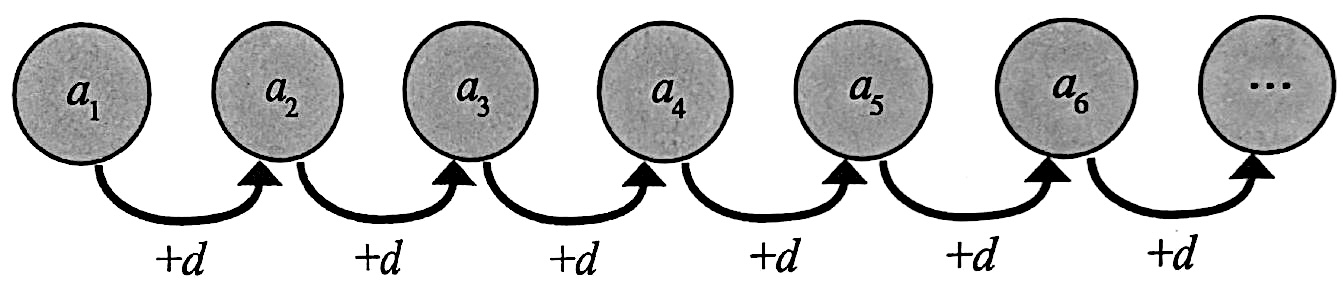
\includegraphics[width=0.5\textwidth]{assets/13-1.jpg}
\end{center}

Let $a_1$ = $a$,
\begin{center}
    \begin{tabular}{|l|l|}
        \hline$a_{1}$ & $a$ \\
        \hline $a_{2}$ & $a_{1}+d=a+d$ \\
        \hline$a_{3}$ & $a_{2}+d=a+2 d$ \\
        \hline$a_{4}$ & $a_{3}+d=a+3 d$ \\
        \hline$a_{5}$ & $a_{4}+d=a+4 d$ \\
        \hline$\cdots$ & $\cdots$ \\
        \hline
    \end{tabular}
\end{center}

From the table above, it can be deduced that if an arithmetic sequence $\left\{a_{n}\right\}$ has a first term $a$ and a common difference $d$, then its general term formula is

\begin{info}[General Term Formula for Arithmetic Sequence]
    $$a_{n}=a+(n-1) d$$
\end{info}

\begin{question}
    Find the 8th term of the arithmetic sequence $1, 5, 9, \cdots$.

    \sol{}

    \noindent First term $a=1$, common difference $d=5-1=4$

    \vspace{-1em}
    \noindent $\therefore$ the 8th term $
        \begin{aligned}[t]
            a_{8}&=a+7 d\\
        & =1+7 \times 4 \\
        & =29
        \end{aligned}
        $
\end{question}

\begin{question}
    Given that the third term of an arithmetic sequence is $-1$ and the seventh term is $-17$. Find the first term, common difference, and the ninth term of this sequence.

    \sol{}
    \noindent $a_{3}=a+2 d=-1\ \cdots\ (1)$

    \vspace{-1em}
    \noindent $a_{7}=a+6 d=-17\ \cdots\ (2)$

    \vspace{-1em}
    \noindent From (1) and $(2)$, we get $d=-4, a=7$

    \vspace{-1em}
    \noindent $a_{9}=a+8 d=7+8(-4)=-25$

    \vspace{-1em}
    \noindent $\therefore$ the first term of this sequence is $7$, the common difference is $-4$, and the ninth term is $-25$.
\end{question}

\begin{question}
    Which term of the arithmetic sequence $-4,-\dfrac{11}{4},-\dfrac{3}{2}, \cdots$ is $16$?

    \sol{}
    \begin{flalign*}
        a&=-4&\\
        d&=a_{2}-a=-\dfrac{11}{4}-(-4)=\dfrac{5}{4}
    \end{flalign*}
    Let's the $n$th term of this arithmetic sequence be $16$, then
    \begin{flalign*}
        a_{n}=a+(n-1) d=-4+\dfrac{5}{4}(n-1) & =16 &\\
        \dfrac{5}{4}(n-1) & =20 \\
        n-1 & =16 \\
        n & =17
    \end{flalign*}
    $\therefore$ the $17$th term of this arithmetic sequence is $16$.
\end{question}

\begin{question}
    How many multiples of 6 are there between 100 and 300?

    \sol{}

    \vspace{-1em}
    \noindent The multiples of 6 from 100 to 300 are $102,108,114, \cdots, 300$.

    \vspace{-1em}
    \noindent They form an arithmetic sequence such that $a=102$ and $d=6$.

    \vspace{-1em}
    \noindent Let the number of terms in this sequence be $n$, then
    \vspace{-0.5em}
    \begin{flalign*}
        a_{n} & =a+(n-1) d &\\
        300 & =102+6(n-1) \\
        \therefore n & =34
    \end{flalign*}

    \vspace{-2em}
    \noindent $\therefore$ there are 34 multiples of 6 between 100 and 300.
\end{question}

\begin{warn}[Keep in Mind:]
    
    \noindent In Example 12, the number of multiples of $6$ does not equal to $(\text{last term} - \text{first term}) \div 6 + 1$.
\end{warn}

The arithmetic mean $A$ of two numbers $x$ and $y$ is the number that forms an arithmetic sequence with $x$ and $y$. Therefore,
$$
\begin{aligned}
& A-x=y-A \\
& \therefore A=\dfrac{x+y}{2}
\end{aligned}
$$
In other words, the arithmetic mean of two numbers is their arithmetic average.

\begin{question}
    Find the arithmetic mean of 3 and 15.

    \sol{}

    The arithmetic mean of 3 and 15 is $\dfrac{3+15}{2}=9$.
\end{question}

\begin{question}
    Find four numbers between 18 and 33 such that these six numbers form an arithmetic sequence.

    \sol{}

    In the targeted arithmetic sequence, $a = 18$
    \begin{flalign*}
        _{6}=a+5 d & =33 &\\
        5 d & =33-18 \\
        d & =3
    \end{flalign*}
    $\therefore$ the four targeted numbers are $21,24,27$, and $30$.
\end{question}

\newpage
\begin{question}
    If the lengths of the sides of a right triangle form an arithmetic sequence, prove that their ratio is $3: 4: 5$.

    \proof{}

    \noindent\textbf{Approach 1:}

    \noindent Suppose $a < b < c$, then $c$ is the hypotenuse. According to the Pythagorean theorem,
    \begin{align*}
        a^2 + b^2 & = c^2\ \cdots\ (1) &&&&&&&&&&&&
    \end{align*}
    Since $a, b, c$ form an arithmetic sequence,
    \begin{align*}
        b &= \dfrac{a+c}{2}\ \cdots\ (2) &&&&&&&&&&&&
    \end{align*}
    Substituting $(2)$ into $(1)$, we get
    \begin{align*}
        a^{2}+\dfrac{a^{2}+2 a c+c^{2}}{4}&=c^{2} &&&&&&&&&&&& \\
        5 a^{2}+2 a c-3 c^{2}&=0 \\
        (5 a-3 c)(a+c)&=0
    \end{align*}
    \vspace{-3.5em}
    \begin{align*}
        \because a+c &\neq 0 &&&&&&&&&&&& \\
        \therefore 5 a-3 c&=0 \\
        a&=\dfrac{3}{5} c
    \end{align*}
    Substituting $a=\dfrac{3}{5} c$ into $(2)$, we get: $b=\dfrac{4}{5} c$.
    
    \vspace{-1em}
    \noindent $\therefore$ the ratio of the lengths of the sides is $3:4:5$.

    \noindent\textbf{Approach 2:}

    \noindent Let the lengths of the sides be $a, a+d$, and $a+2d$, where $d>0$, then $a+2d$ is the length of the hypotenuse. By the Pythagorean theorem,
    \begin{align*}
    a^{2}+(a+d)^{2}&=(a+2 d)^{2} &&&&&&&&&&&& \\
    a^{2}-2 a d-3 d^{2}&=0 \\
    (a-3 d)(a+d)&=0
    \end{align*}
    \vspace{-3.5em}
    \begin{align*}
    \because a+d &\neq 0 &&&&&&&&&&&& \\
    \therefore a-3 d&=0 \\
    a&=3 d
    \end{align*}
    $\because$ the lengths of the sides are $3 d, 4 d$, and $5 d$.

    \vspace{-1em}
    \noindent $\therefore$ the ratio of the lengths of the sides is $3:4:5$.
\end{question}

\practice{13.2a}
\begin{enumerate}
    \item Given that the 4th term and the 9th term of an arithmetic sequence are -2 and 28 respectively, find the first term, common difference, and the 12th term of this sequence.
    \item Find the arithmetic mean of -9 and 21.
    \item Find five numbers between -40 and 56 such that these seven numbers form an arithmetic sequence.
    \item How many multiples of 7 are there between 100 and 1000?
\end{enumerate}

\subsection*{Sum of the First \(n\) Terms}

If \(a_{1}, a_{2}, a_{3}, \cdots, a_{n}\) is an arithmetic sequence, the expression obtained by adding the terms of the sequence, \(a_{1}+a_{2}+\cdots+a_{n}\), is called an \textbf{arithmetic series}. We usually denote the sum of the first \(n\) terms of a sequence \(\{a_{n}\}\) and its corresponding series \(a_{1}+a_{2}+\cdots+a_{n}+\cdots\) as \(S_{n}\), that is,
$$
S_{n}=a_{1}+a_{2}+\cdots+a_{n}
$$

\vspace{-1em}
The great mathematician Gauss, at the age of $8$, already knew a quick method to find the sum of the arithmetic sequence \(1, 2, 3, \cdots, 100\). His idea was as follows:
\begin{center}
    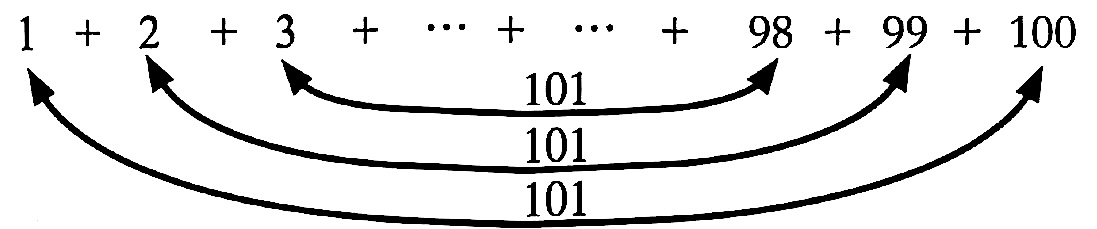
\includegraphics[width=0.5\textwidth]{assets/13-2.jpg}
\end{center}

Pairing \(1, 2, 3, \cdots, 100\) from the beginning and end, we can divide them into $50$ pairs, and the sum of each pair is $101$. Therefore,
$$
1+2+3+\cdots+98+99+100=50 \times 101=5050
$$

\vspace{-1em}
By generalizing this idea, we can derive the formula for the sum of an arithmetic sequence. Let \(S_{n}\) be the sum of the first \(n\) terms of an arithmetic sequence \(\{a_{n}\}\),
\begin{center}
    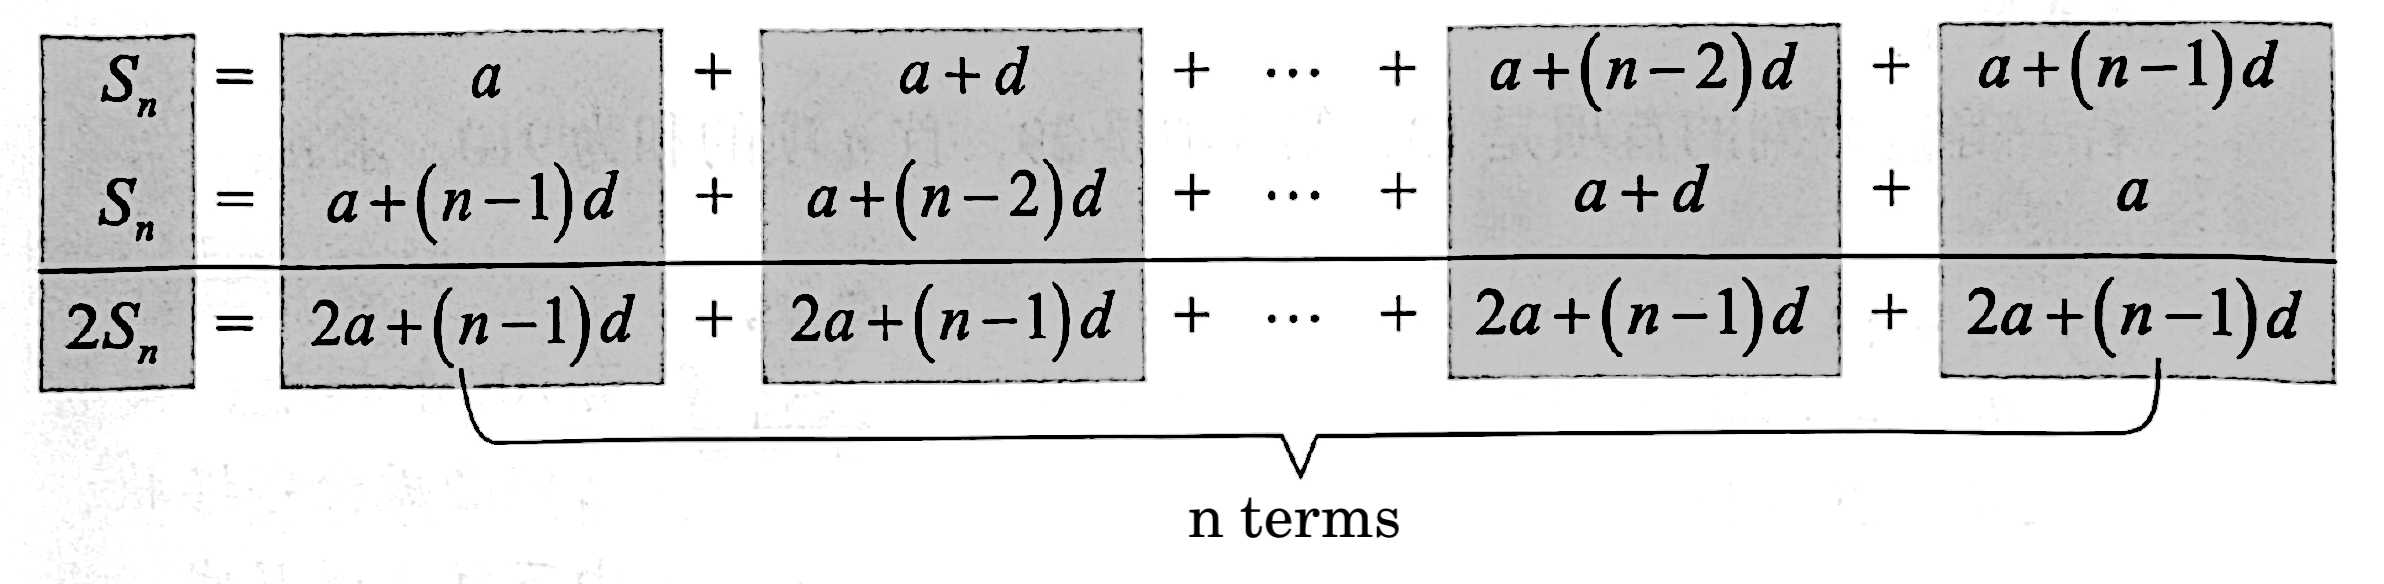
\includegraphics[width=0.7\textwidth]{assets/13-3.png}
\end{center}
\vspace{-2em}
$$
2 S_{n}=n[2 a+(n-1) d]
$$
Hence,
\begin{info}[Sum of the First \(n\) Terms of an Arithmetic Sequence]
    $$S_{n}=\dfrac{n}{2}\left[2 a+(n-1) d\right]$$
\end{info}
Since \(2a + (n-1)d\) is the sum of the first and last terms, this formula for the sum can also be written as
\begin{info}[Sum of the First \(n\) Terms of an Arithmetic Sequence]
    $$S_{n}=\dfrac{n}{2}(a_{1}+a_{n})$$
\end{info}

\begin{question}
    Find the sum of all multiples of $4$ from $50$ to $500$.

    \sol{}

    \noindent From $50$ to $500$, all multiples of $4$ are \(52, 56, \cdots, 500\). They form an arithmetic sequence.

    \vspace{-1em}
    \noindent $a=52, d=4$,

    \vspace{-1em}
    \noindent There are a total of $n=\dfrac{500-52}{4}+1=113$ terms

    \vspace{-1em}
    \noindent $\therefore$ the sum of all multiples of $4$ from $50$ to $500$ is \(S_{113} = \dfrac{113}{2}(52+500) = 31188\).
\end{question}
\vspace{-2em}
\begin{question}
    If the first term of an arithmetic sequence is $13$, the third term is $29$, and the sum of the first \(n\) terms is $910$, find \(n\).

    \sol{}
    \begin{flalign*}
        a & =13 &\\
        a_3 & =a+2 d=29 \\
        2 d & =29-13 \\
        d & =8
    \end{flalign*}
    \vspace{-3.5em}
    \begin{flalign*}
        S_n=\dfrac{n}{2}[2 \times 13+8(n-1)] & =910 &\\
        n(4 n+9) & =910 \\
        4 n^2+9 n-910 & =0 \\
        (n-14)(4 n+65) & =0
    \end{flalign*}
    $\because n > 0$

    \vspace{-1em}
    \noindent $\therefore n=14$
\end{question}

    \begin{multicols}{2}
    \begin{think}

        \noindent If you precisely stack all 100 cups into a pyramid shape, one by one, starting from the bottom and moving up, will you use up all of them?
    \end{think}

        \begin{center}
            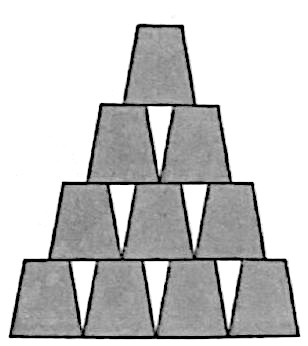
\includegraphics[width=0.2\textwidth]{assets/13-4.jpg}
        \end{center}
    \end{multicols}

    \begin{question}
        At which term of the arithmetic progression $-56, -50, -44, \ldots$ does the sum become positive when adding from the first term?

        \sol{}
        \begin{flalign*}
            a=-56, d=-50-(-56) & =6 &\\
            S_n=\dfrac{n}{2}[2(-56)+6(n-1)] & >0 \\
            n(3 n-59) & >0\\
                \because n>0, \therefore 3 n-59&>0 \\
                n&>19 \dfrac{2}{3}
        \end{flalign*}
        $\therefore$ you must add from the first term to the $20^{th}$ term for the sum to become positive.
    \end{question}

    \vspace{-1.5em}
    \begin{question}
        Given a sequence $\left\{a_{n}\right\}$ with the sum of its first $n$ terms being $S_{n}=2 n^{2}+3 n$,
        \begin{tasks}[label=(\alph*)]
            \task Find the first term of the sequence $a_{1}$.
            \task Find the general formula for the sequence $a_{n}$.
            \task Prove that $\left\{a_{n}\right\}$ is an arithmetic sequence.
            \task Find the sum of the sequence from the 5th term to the 12th term.
        \end{tasks}

        \sol{}
        \begin{tasks}[label=(\alph*)]
            \task $a_{1}=S_{1}=2(1)^{2}+3(1)=5$
            
            \task $\begin{aligned}[t]
                S_n & =a_1+a_2+\cdots+a_{n-1}+a_n \\
                S_{n-1} & =a_1+a_2+\cdots+a_{n-1}
            \end{aligned}$
            \vspace{-1em}
            \begin{flalign*}
                \therefore a_n & =S_n-S_{n-1} &\\
                & =2 n^2+3 n-\left[2(n-1)^2+3(n-1)\right] \\
                & =4 n+1
            \end{flalign*}
            \vspace{-2em}
            
            \task $\begin{aligned}[t]
                &a_{n-1}=4(n-1)+1=4 n-3\\
                &\therefore a_n-a_{n-1}=4 \text{ is a constant}\\
                &\therefore\left\{a_n\right\} \text{ is an arithmetic sequence}
            \end{aligned}$

            \task Sum of the sequence from the 5th term to the 12th term 
            
            $\begin{aligned}[t]
                & =a_5+a_6+\cdots+a_{12} \\
                & =\left(a_1+a_2+\cdots+a_{12}\right)-\left(a_1+a_2+a_3+a_4\right) \\
                & =S_{12}-S_4 \\
                & =2(12)^2+3(12)-\left[2(4)^2+3(4)\right] \\
                & =280
                \end{aligned}
            $
        \end{tasks}
    \end{question}

    \begin{info}[Additional Information:]
        
        \noindent From the solution to Example 19, it can be observed that if the sum of the first $n$ terms of a sequence $\left\{a_{n}\right\}$ is $S_{n}$, then:
        \vspace{-1em}
        \begin{itemize}[leftmargin=*]
            \item The $n$th term is given by $a_{n}=S_{n}-S_{n-1}$.
            \item The sum of the terms from the $k$th term to the $l$th term is $S_{l}-S_{k-1}$.
        \end{itemize}
    \end{info}

    \begin{question}
        Given that the first term of an arithmetic sequence is 13, and the sum of its first 4 terms equals the sum of its first 10 terms, find the value of $n$ when the sum of the first $n$ terms reaches its maximum.

        \sol{}
        \begin{flalign*}
            a & =13 &\\
            S_4 & =S_{10} \\
            \dfrac{4}{2}(2 \times 13+3 d) & =\dfrac{10}{2}(2 \times 13+9 d) \\
            52+6 d & =130+45 d \\
            39 d & =-78 \\
            d & =-2
        \end{flalign*}
        \vspace{-3.5em}
        \begin{flalign*}
            S_n & =\dfrac{n}{2}[2 \times 13-2(n-1)] &\\
            & =n(14-n) \\
            & =-\left(n^2-14 n+49\right)+49 \\
            & =49-(n-7)^2
        \end{flalign*}
        $\therefore$ When $n=7$, the sum of the first $n$ terms reaches its maximum.
    \end{question}

    \begin{think}
        
        \noindent In Example 20, do you expect the answer to be $7$ before any calculation? Why would you have such a thought?
    \end{think}

    \newpage
    \practice{13.2b}
    \begin{enumerate}
        \item On the "$365$-Day Savings Plan," you start by saving RM $0.10$ on the first day, RM $0.20$ on the second day, RM $0.30$ on the third day, increasing by RM $0.10$ each day, for a total of $365$ days. How much money will you have saved after $365$ days?
        
        \item Given that the $3^{rd}$ term of an arithmetic sequence is $24$, the $15^{th}$ term is $-12$, and the sum of the first $n$ terms is $30$, find the value of $n$.
    
        \item Given that the sum of the first $n$ terms of a sequence $\left\{a_{n}\right\}$ is $S_{n}=\dfrac{4 n-3 n^{2}}{2}$.
        \begin{enumerate}
            \item Find the $n$th term $a_{n}$ of the sequence.
            \item Find the sum of the sequence from the $8^{th}$ term to the $15^{th}$ term.
        \end{enumerate}
    \end{enumerate}

    \exercise{13.2}
    \begin{enumerate}
        \item Find the $10^{th}$ term and the $n$th term of the arithmetic sequence $5, 13, 21, \cdots$.
        \item Given that the first term of an arithmetic sequence is $\dfrac{13}{3}$, the $3^{rd}$ term is $3$, and the last term is $-\dfrac{31}{3}$, find the number of terms.
        \item Given that the $7^{th}$ term of an arithmetic sequence is $-10$, and the $12^{th}$ term is $-25$, find the $17^{th}$ term of this sequence.
        \item Given that the $6^{th}$ term of an arithmetic sequence is $43$, the $10^{th}$ term is $75$, find which term is $155$.
        \item Find five numbers between $18$ and $30$ such that these seven numbers form an arithmetic sequence, then find the sum of these $7$ numbers.
        \item Given that the first term of an arithmetic sequence is $12$, and the $2^{nd}$ term is $15$, find the sum of the first $20$ terms.
        \item Given that the first term of an arithmetic sequence is $20$, and the third term is $\dfrac{92}{5}$, find which term is the first negative term.
        \item Given that three numbers form an arithmetic sequence, and their sum is $30$, and the sum of their squares is $318$, find these three numbers.
        \item Find the sum of the first $12$ terms of the arithmetic series $18, 10, 2, -6, \cdots$.
        \item  If the $4^{th}$ term of an arithmetic sequence is $9$, and the 8th term is $-7$, find the sum of its first $10$ terms.
        \item  Find the sum of all integers between $200$ and $800$ that are divisible by $11$.
        \item  Given that the first three terms of an arithmetic sequence are $x, 3x-4, 2x+7$.
        \begin{enumerate}
            \item Find the value of $x$.
            \item Find the sum of the first $10$ terms of this sequence.
        \end{enumerate}
        \item Given that the first term of an arithmetic sequence is $12$, the common difference is $-3$, and the sum of all terms is $21$, find the number of terms.
        \item Given that the $3^{rd}$ term of an arithmetic sequence is $8$, and the $6^{th}$ term is $4$. Starting from the first term, up to which term must we add to get a negative sum?
        \item Given that the sum of the first $n$ terms of a sequence is $S_{n}=\dfrac{n(n+3)}{4}$.
        \begin{enumerate}
            \item Find the first term $a_{1}$ of the sequence.
            \item Find the general formula $a_{n}$ of the sequence.
            \item Prove that $\left\{a_{n}\right\}$ is an arithmetic sequence.
            \item Find the sum of the sequence from the $8^{th}$ term to the $22^{nd}$ term.
        \end{enumerate}

        \item Refer to the image below:
        \begin{center}
            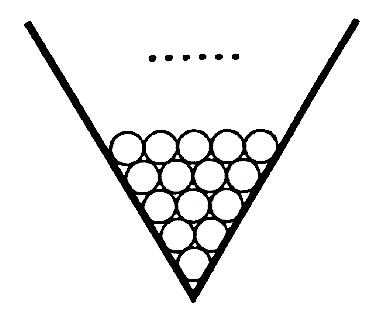
\includegraphics[width=0.2\textwidth]{assets/13-5.jpg}
        \end{center}
        \begin{enumerate}
            \item If there are $50$ pencils in the top layer, how many pencils are there in total?
            \item If there are $990$ pencils in total, how many layers are there?
        \end{enumerate}
        \item Given that the first term of an arithmetic sequence is positive, and the $20^{th}$ term is $0$. If the sum of the first $n$ terms of this sequence is $0$, find the value of $n$.
        \item Given that the $5^{th}$ term of an arithmetic sequence is $3$, and the sum of the first $10$ terms is $26 \dfrac{1}{4}$, find which term has the value $0$.
        \item Let $S_{n}$ be the sum of the first $n$ terms of an arithmetic sequence $\left\{a_{n}\right\}$. If $S_{10}=465$ and $9 S_{3}=4 S_{6}$, find $a_{5}$ and $S_{5}$.
        \item Find $38^{2}-37^{2}+36^{2}-35^{2}+\cdots+2^{2}-1^{2}$.
        \item Given that the first term of an arithmetic sequence is $45$, and the common difference is $-6$, for what value of $n$ does the sum $S_{n}$ of the first $n$ terms reach its maximum?
        \item Given that the interior angles of a convex polygon form an arithmetic sequence with a common difference of 6, and the largest interior angle is $135^{\circ}$. How many sides does this polygon have?
        \item Given that the sum of the first 6 terms of an arithmetic sequence is 96, and the sum of the first 10 terms is one-third of the sum of the first 20 terms, find the first term and the 10th term of this sequence.
        \end{enumerate}

        \newpage
        \section{Geometric Sequence and Series}

        When each term of a sequence $\left\{a_{n}\right\}$ is equal to the ratio of the term and its preceding term, this sequence is called a \text{geometric sequence}, and this equal ratio is called the \text{common ratio}, generally denoted by $r$. According to the definition,
        $$
            \dfrac{a_{n}}{a_{n-1}}=r
        $$
        Hence,
        $$
            a_{n}=a_{n-1} \times r
        $$
        \begin{center}
            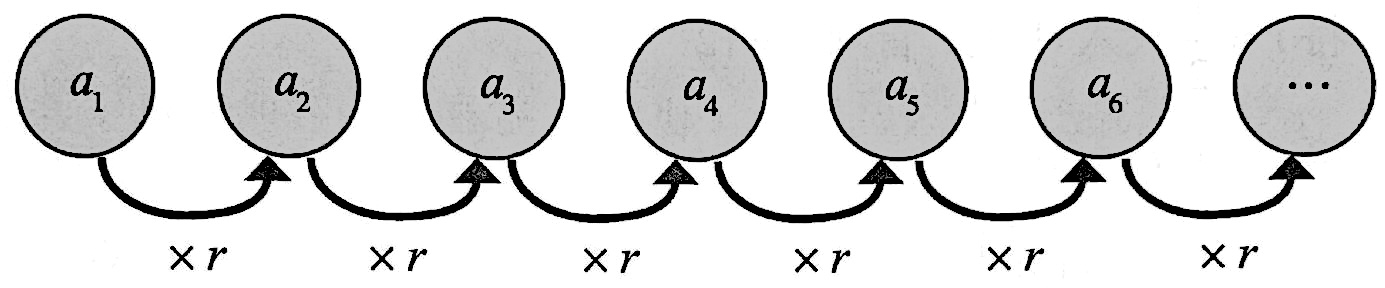
\includegraphics[width=0.5\textwidth]{assets/13-6.jpg}
        \end{center}
        
        Let $a_{1}=a$,
        \begin{center}
            \begin{tabular}{|l|l|}
                \hline$a_{1}$ & $a$ \\
                \hline $a_{2}$ & $a_{1} \times r=ar$ \\
                \hline$a_{3}$ & $a_{2} \times r=ar^{2}$ \\
                \hline$a_{4}$ & $a_{3} \times r=ar^{3}$ \\
                \hline$a_{5}$ & $a_{4} \times r=ar^{4}$ \\
                \hline$\cdots$ & $\cdots$ \\
                \hline
            \end{tabular}
        \end{center}
        From the table above, it can be deduced that if a geometric sequence $\left\{a_{n}\right\}$ has a first term of $a$ and a common ratio of $r$, then its general term formula is
        $$
            a_{n}=a r^{n-1}
        $$

        \begin{question}
            Given that the second term and the fifth term of a geometric sequence are $6$ and $\dfrac{3}{4}$ respectively, find its first term and the tenth term.

            \sol{}
            \begin{flalign*}
                a_2 &= ar = 6\ \cdots\ (1) &\\
                a_5 &= ar^4 = \dfrac{3}{4}\ \cdots\ (2)
            \end{flalign*}
            $\dfrac{(2)}{(1)}$ gives $\qquad\begin{aligned}[t]
                r^3 & =\dfrac{1}{8} \\
                r & =\dfrac{1}{2}
            \end{aligned}$
            Substituting $r=\dfrac{1}{2}$ into $(1)$, we get $a=12$.

            \vspace{-1em}
            \noindent The $10^{th}$ term $\begin{aligned}[t]
                a_{10} & = a r^{9} = 12\left(\dfrac{1}{2}\right)^9 = \dfrac{3}{128}
            \end{aligned}$
        \end{question}

        \begin{question}
            The $2^{nd}$ of a geometric sequence is $-8$, and the $3^{rd}$ is $4$. What is the term number where the value is $\dfrac{1}{1024}$?

            \sol{}
            \vspace{-1em}
            \begin{flalign*}
                a_2 & =ar=-8\ \cdots\ (1) &\\
                a_3 & =ar^2=4\ \cdots\ (2)
            \end{flalign*}
            $\dfrac{(2)}{(1)}$ gives $\qquad\begin{aligned}[t]
                r & =-\dfrac{1}{2},\ a & =16
            \end{aligned}$

            \noindent Let the $n^{th}$ term be $\dfrac{1}{1024}$, then
            \begin{flalign*}
                a_n=a r^{n-1} & =16\left(-\dfrac{1}{2}\right)^{n-1} \\
                \dfrac{1}{1024} & =\dfrac{16}{(-2)^{n-1}} \\
                (-2)^{n-1} & =(-2)^{14} \\
                n & =15 &
            \end{flalign*}

            \vspace{-2.5em}
            $\therefore$ the $15^{th}$ term is $\dfrac{1}{1024}$.
        \end{question}

        \vspace{-1.5em}
        The geometric mean $G$ of two numbers $x$ and $y$ is a number that forms a geometric sequence with $x$ and $y$. Hence,
        $$
        \begin{aligned}
        \dfrac{G}{x} & =\dfrac{y}{G} \\
        G^{2} & =x y \\
        \therefore G & = \pm \sqrt{x y}
        \end{aligned}
        $$

        \vspace{-1em}
        If $x$ and $y$ are both positive numbers, then $\sqrt{xy}$ is their geometric mean.

        \begin{think}
            
            \noindent Two numbers $x$ and $y$ must have the same sign to have a geometric mean. Why?
        \end{think}
        \vspace{1em}

        \begin{question}
            Find three numbers between $\dfrac{1}{6}$ and $216$ such that these five numbers form a geometric sequence.

            \sol{}

            \vspace{-1em}
            \noindent In the targeted geometric sequence, $a=\dfrac{1}{6}$
            \vspace{-1em}
            \begin{align*}
                a_5&=a r^4=216 &&&&&&&&&&&& \\
                r^4&=216 \times 6=6^4 \\
                r&= \pm 6
            \end{align*}

            \vspace{-2em}
            \noindent $\therefore$ the three targeted numbers are $1, 6, 36$ or $-1, 6, -36$.
        \end{question}

        \begin{question}
            Given that the population of Malaysia was $28.33$ million people in $2010$ and $29.72$ million people in $2013$:
            \begin{tasks}[label=(\alph*)]
                \task Find the annual growth rate of Malaysia's population during this period.
                \task Estimate the population of Malaysia in $2020$.
            \end{tasks}

            \sol{}
            \begin{tasks}[label=(\alph*)]
                \task Let $a_{1}$ be the population in 2010 (in tens of millions of people), $a_{2}$ be the population in 2011, and so on.
                \begin{align*}
                    a_1=a &= 2833 &&&&&&&&&&&& \\
                    a_4=a r^3 & =2972 \\
                    r^3 & =\dfrac{2972}{2833} \\
                    r & =\sqrt[3]{\dfrac{2972}{2833}} \\
                    & =1.0161
                \end{align*}
                $\therefore$ the annual growth rate of Malaysia's population is $(1.0161-1) \times 100 \% = 1.61 \%$.

                \task In the year $2020$, the population of Malaysia will be $
                a_{11}=a r^{10}=2833 \times 1.0161^{10}=33.24 \text { million }
                $
            \end{tasks}
        \end{question}

        \vspace{-2em}
        \practice{13.3a}
        \begin{enumerate}
            \item The first term of a geometric sequence is $18$, and the second term is $12$. Find the sixth term.

            \item The first term of a geometric sequence is $8$, and the fourth term is $-27$. What term is $-\dfrac{2187}{16}$ located at?
            
            \item Find the geometric mean of $\dfrac{27}{8}$ and $\dfrac{2}{3}$.
        \end{enumerate}

        \vspace{-1em}
        \exercise{13.3a}
        \begin{enumerate}
            \item Given that the first term of a geometric sequence is $8$, the second term is $4$, and the last term is $\dfrac{1}{128}$, find the number of terms.

            \item  Given that the second term of a geometric sequence is $12$ and the fourth term is $108$, find the seventh term.
            
            \item Insert three numbers between $14$ and $224$ to form a geometric sequence with these five numbers.
            
            \item Given that the seventh term of a geometric sequence is $18$ and the common ratio is $-\dfrac{3}{2}$, find the fourth term.
            
            \item If $x+12$, $x+4$, and $x-2$ form a geometric sequence, find the value of $x$ and the common ratio of the sequence.
            
            \item Given that the second, sixth, and eighth terms of an arithmetic sequence form a geometric sequence, find the common ratio of this geometric sequence.
            
            \item Three different numbers $2$, $x$, and $y$ form a geometric sequence. If these three numbers are the first, second, and twelfth terms of an arithmetic sequence, find the values of $x$ and $y$.
        \end{enumerate}

        \subsection*{Sum of the First \(n\) Terms}

        If $a_{1}, a_{2}, a_{3}, \cdots, a_{n}$ is a geometric sequence, then the expression obtained by adding all the terms in the sequence $a_{1}+a_{2}+\cdots+a_{n}$ is called a \text{geometric series}. Let $S_{n}$ be the sum of the first $n$ terms of a geometric sequence $\left\{a_{n}\right\}$.
        \vspace{-1em}
        \begin{center}
            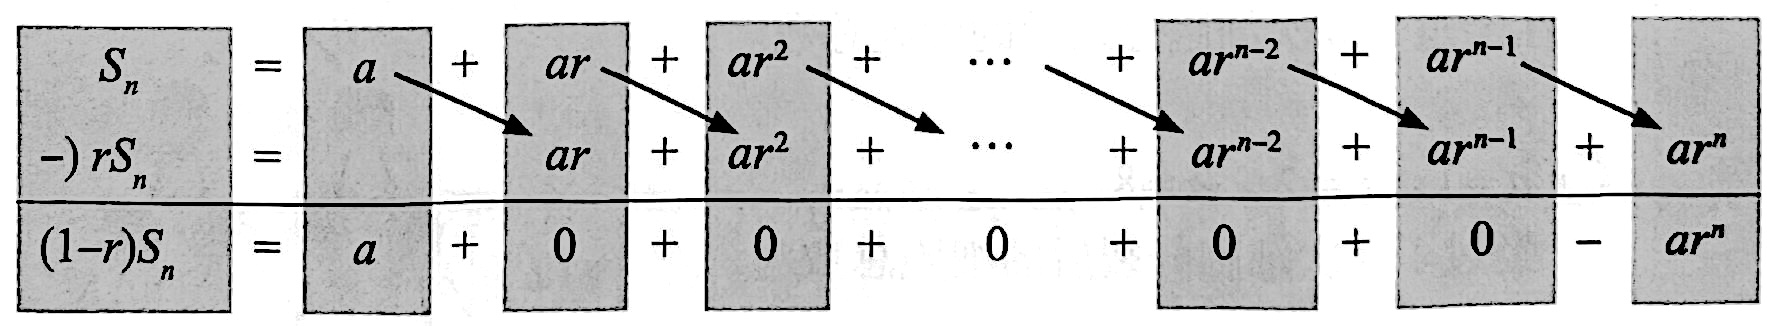
\includegraphics[width=0.7\textwidth]{assets/13-7.jpg}
        \end{center}
        \vspace{-1em}
        $\therefore(1-r) S_{n}=a\left(1-r^{n}\right)$
        
        From this, it follows that when $r \neq 1$, the sum formula for a geometric series is:
        \begin{info}[Sum of the First \(n\) Terms of a Geometric Sequence]
            $$
            S_{n}=\dfrac{a(1-r^{n})}{1-r}
            $$
        \end{info}
        
        When $r=1$, the resulting geometric sequence is a constant sequence $a, a, a, \cdots$. Clearly, in this case, the sum of the first $n$ terms of the sequence is $S_{n}=n a$.
        
        \begin{question}
            Find the sum of the first $7$ terms of the geometric series $2-3+\dfrac{9}{2}-\cdots$.

            \sol{}

            \noindent $a = 2$, $r = \dfrac{-3}{2} = -\dfrac{3}{2}$

            \vspace{-1em}
            \noindent $\therefore$ Sum of the first $7$ terms $S_{7}=\dfrac{2\left[1-\left(-\dfrac{3}{2}\right)^{7}\right]}{1-\left(-\dfrac{3}{2}\right)}=\dfrac{463}{32}$.
        \end{question}

        \begin{question}
            If during the process of cell division, one cell divides into two, find the total number of cells after $8$ rounds of cell division.

            \sol{}
            \vspace{-1.5em}
            \begin{multicols}{2}
            \noindent $a = 1$, $r = 2$, $n = 8$

            \vspace{-1em}
            \noindent The total number of cells after $8$ rounds of cell division is
            \begin{flalign*}
                S_9 & =\dfrac{1 \times\left(1-2^8\right)}{1-2}& \\
                & =255
            \end{flalign*}
            \columnbreak

            \begin{center}
                \vspace*{-3em}
                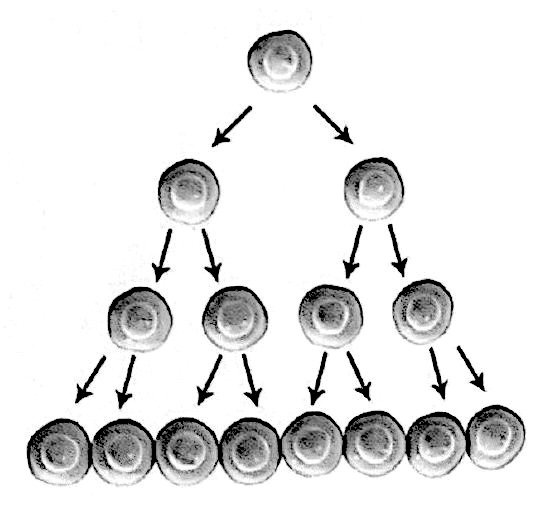
\includegraphics[width=0.25\textwidth]{assets/13-8.jpg}
            \end{center}
            \end{multicols}
            \vspace{-4em}
        \end{question}

        \begin{question}
            Given that all terms of a geometric sequence are positive, the second term is $72$, and the fourth term is $32$. Find the value of $n$ such that the sum of the first $n$ terms is $281 \dfrac{1}{3}$.

            \sol{}
            \begin{flalign*}
                a_2 &= ar = 72\ \cdots\ (1) &\\
                a_4 &= ar^3 = 32\ \cdots\ (2)
            \end{flalign*}
            $\dfrac{(2)}{(1)}$ gives $\qquad\begin{aligned}[t]
                r^2 & =\dfrac{32}{72} =\dfrac{4}{9} \\
            \end{aligned}$
            
            \noindent Since all the terms in this geometric sequence are positive, $r>0$,
            \begin{align*}
                \therefore\ r = \dfrac{2}{3},\ a &= \dfrac{72}{\dfrac{2}{3}} = 108 &&&&&&&&&&&&
            \end{align*}
            \vspace{-2em}
            \begin{flalign*}
                S_n=\dfrac{108\left[1-\left(\dfrac{2}{3}\right)^n\right]}{1-\dfrac{2}{3}} & =\dfrac{844}{3} \\
                1-\left(\dfrac{2}{3}\right)^n & =\dfrac{211}{243} \\
                \left(\dfrac{2}{3}\right)^n & =\dfrac{32}{243}=\left(\dfrac{2}{3}\right)^5 \\
                \therefore n & =5 &
            \end{flalign*}
        \end{question}

        \begin{question}
            Given that the first term of an arithmetic sequence is $-3$, and its $4^{th}$, $6^{th}$, and $10^{th}$ terms are the $2^{nd}$, $3^{rd}$, and $4^{th}$ terms of a geometric sequence, respectively. If the arithmetic sequence is not a constant sequence,
            \vspace{-1em}
            \begin{enumerate}[label=(\alph*)]
                \item Find the common difference of the arithmetic sequence.

                \item Find the sum of the first $10$ terms of the geometric sequence.
            \end{enumerate}

            \sol{}
            \vspace{-1em}
            \begin{enumerate}[label=(\alph*)]
                \item The $4^{th}$, $6^{th}$, and $10^{th}$ terms of the arithmetic sequence are $-3+3d$, $-3+5d$, and $-3+9d$ respectively.

                $\because$ they are three consecutive terms of a geometric sequence
    
                $\begin{aligned}
                    \therefore(-3+3 d)(-3+9 d) & =(-3+5 d)^2 \\
                    2 d^2-6 d & =0 \\
                    2 d(d-3) & =0
                    \end{aligned}$
    
                    $\because$ the arithmetic sequence is not a constant sequence, $d \neq 0$
    
                    $\therefore d=3$
            \end{enumerate}
        \end{question}

        \setcounter{Question}{27}
        \begin{question}
            \begin{enumerate}[label=(\alph*), start=2]
                \item The $2^{nd}$, $3^{rd}$, and $4^{th}$ terms of the geometric sequence are $6$, $12$, and $24$ respectively.
                    \begin{align*}
                        \text{Common ratio } r &= \dfrac{12}{6} = 2 &&&&&&&&&&&& \\
                        \text{First term } a &= \dfrac{6}{2} = 3
                    \end{align*}
                    $\therefore$ The sum of the first $10$ terms $S_10 = \dfrac{3(1-2^{10})}{1-2} = 3069$.
            \end{enumerate}
        \end{question}

        \practice{13.3b}
        \begin{enumerate}
            \item Find the sum of the series $\dfrac{1}{2}+\dfrac{1}{4}+\dfrac{1}{8}+\cdots+\dfrac{1}{2^{n}}$.

            \item Given that the first term of a geometric series is $2$, the fourth term is $-128$, and the last term is $8192$, find the sum of this series.
            
            \item A ball falls from a height of 18 m. After each bounce, it rebounds to $\dfrac{2}{3}$ of its previous height. Find the total distance traveled by the ball from the start to the fourth bounce.
            
            \item In the Chinese mathematical masterpiece "Suanfa Tongzong," there is the following problem:
            
            "Looking afar, a towering seven-story pagoda, dots of red light increasingly bright, a total of 381 lamps, please tell me how many lamps are at the top?"
            
            Meaning: A seven-story pagoda has a total of $381$ lamps. The number of lamps on the next lower level is twice the number on the level above. Find the number of lamps at the top level of the pagoda. Can you figure it out?
        \end{enumerate}

        \section*{Sum of an Infinite Geometric Series}
        \begin{center}
            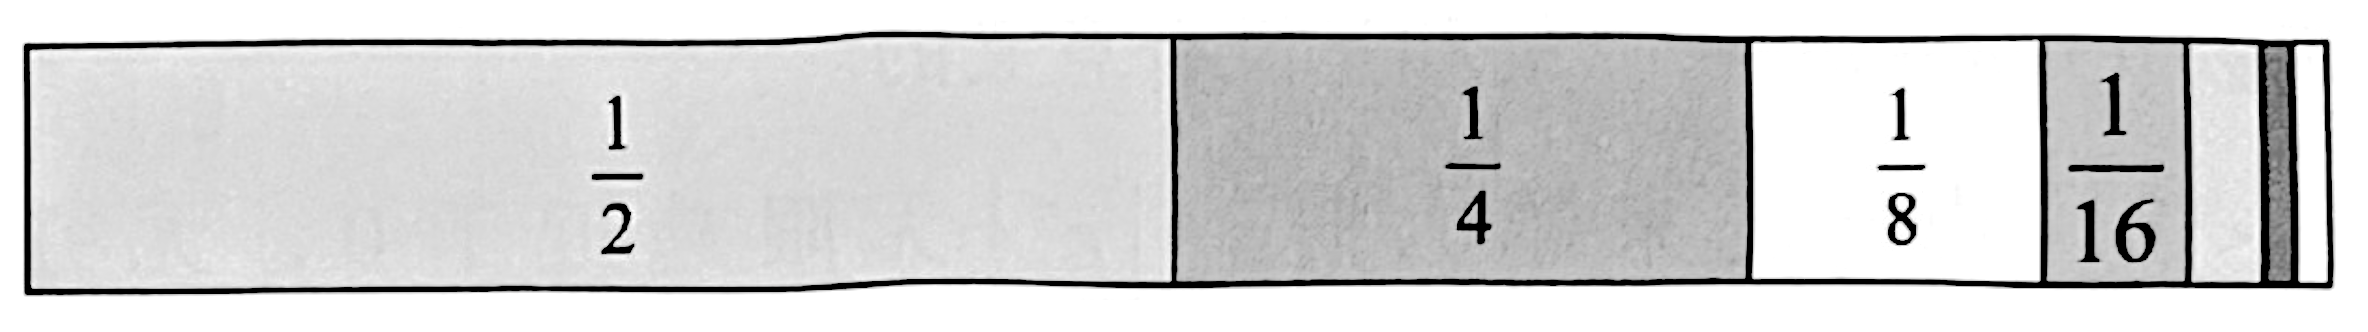
\includegraphics[width=0.7\textwidth]{assets/13-9.png}    
        \end{center}
        
        We can imagine the ribbon in the figure above as a ribbon of length 1. Initially, we cut off $\dfrac{1}{2}$ of the ribbon, then we cut off $\dfrac{1}{4}$ from the remaining $\dfrac{1}{2}$, which is $\dfrac{1}{4}$ of the original length, and so on. Each time we cut off a ribbon whose length is $\dfrac{1}{2}$ of the remaining ribbon. Therefore, after the $n$th cut, the length of the ribbon cut off is $\dfrac{1}{2^n}$, leaving $\dfrac{1}{2^n}$ of the ribbon.

        Hence, the total length of ribbon cut off after $n$ cuts is the sum of the infinite series $\dfrac{1}{2}+\dfrac{1}{4}+\dfrac{1}{8}+\cdots+\dfrac{1}{2^n}+\cdots$. Obviously, this sum equals 1, i.e.,
        $$
        \dfrac{1}{2}+\dfrac{1}{4}+\dfrac{1}{8}+\cdots+\dfrac{1}{2^n}+\cdots=1
        $$

        \vspace{-1em}
        Mathematically, we say that the sum of the first $n$ terms of this infinite series is $1-\dfrac{1}{2^n}$. As $n$ approaches infinity, since $\dfrac{1}{2^n}$ tends to $0$, the sum of the first $n$ terms approaches $1$. Therefore, we say that $1$ is the sum of the infinite series $\dfrac{1}{2}+\dfrac{1}{4}+\dfrac{1}{8}+\cdots+\dfrac{1}{2^n}+\cdots$.

        For a geometric series $a+ar+ar^2+\cdots+ar^n+\cdots$,
        \begin{itemize}
            \item When $r \neq 1$, the sum of its first $n$ terms is $S_{n}=\dfrac{a(1-r^n)}{1-r}$.

            \item When $r=1$, $S_{n}=na$.
            
            \item If $a \neq 0$, when $r=-1$, $S_{n}=\left\{\begin{array}{l}a, \text { if } n \text { is odd } \\ 0, \text { if } n \text { is even }\end{array}\right.$.
        \end{itemize}
        
        \begin{think}
            
            \noindent Does it make sense to sum an infinite series with an arithmetic progression?
        \end{think}

        For an infinite geometric series $a+ar+ar^2+\cdots$, when $|r| \geq 1$, as more terms are added, the sum does not converge to any constant value. Therefore, we say the sum of the infinite geometric series $a+ar+ar^2+\cdots$ is undefined.

        If $|r|<1$, as $n$ becomes larger, $\left|r^{n}\right|$ approaches $0$, and the sum of the first $n$ terms of the infinite geometric series $a+ar+ar^2+\cdots$, denoted as $S_{n}=\dfrac{a\left(1-r^{n}\right)}{1-r}$, approaches $\dfrac{a}{1-r}$. Therefore, the sum of the infinite geometric series $a+ar+ar^2+\cdots$ is
        
        \begin{info}[Sum of an Infinite Geometric Series]
            $$
            S=\dfrac{a}{1-r} \qquad(-1<r<1)
            $$
        \end{info}

        \begin{info}[Additional Information:]
            
            \noindent In "Zhuangzi," there is a saying:

            \noindent "A one-foot stick, if you take half of it each day, will never be exhausted for ten thousand generations."
        \end{info}        
        
        \begin{question}
            Given that the $3^{rd}$ and $6^{th}$ terms of an infinite geometric series are $^{21}$ and $-\dfrac{56}{9}$ respectively, find the sum of this series.

            \sol{}
            \begin{flalign*}
                a_3 & =ar^2=\dfrac{21}{9}\ \cdots\ (1) &\\
                a_6 & =ar^5=-\dfrac{56}{9}\ \cdots\ (2)
            \end{flalign*}
            $\dfrac{(2)}{(1)}$ gives $\qquad\begin{aligned}[t]
                r^3 & =-\dfrac{8}{27} = \left(-\dfrac{2}{3}\right)^3 \\
                r & =-\dfrac{2}{3}\\
                a & =\dfrac{21}{\left(-\dfrac{2}{3}\right)^2} = \dfrac{189}{4}
            \end{aligned}$

            \vspace{-1em}
            \noindent $\therefore$ the sum of this series $S=\dfrac{a}{1-r}=\dfrac{\dfrac{189}{4}}{1-\left(-\dfrac{2}{3}\right)}=\dfrac{567}{20}$.
        \end{question}

        \vspace{-1em}
       Back in junior high, we learned that any fraction can be expressed as a finite decimal or a repeating decimal. For example:
        $$
        \begin{aligned}
        & \dfrac{15}{8}=1.875 \\
        & \dfrac{1}{6}=0.1666 \cdots=0.16
        \end{aligned}
        $$

        \vspace{-1em}
        Clearly, any finite decimal can be converted into a fraction. As for repeating decimals, we can use the formula for the sum of an infinite geometric series to convert them into fractions, as demonstrated in the following examples.

        \begin{question}
            Convert the repeating decimal $0.2 \dot{1}\dot{3}$ into a fraction.

            \sol{}
            
            \noindent $0.2 \dot{1}\dot{3}=0.2 + (0.013 + 0.00013 + 0.0000013 + \cdots)$
            
            \vspace{-1em}
            \noindent $0.013 + 0.00013 + 0.0000013 + \cdots$ is an infinite geometric series with the first term $a=0.013$, and the common ratio $r=00.1$.
            \begin{flalign*}
                \therefore 0.2 \dot{1} \dot{3} & =0.2+\dfrac{0.013}{1-0.01} \\
                & =0.2+\dfrac{0.013}{0.99} \\
                & =\dfrac{2}{10}+\dfrac{13}{990} &\\
                & =\dfrac{211}{990}
            \end{flalign*}
        \end{question}

        \practice{13.3c}
        \begin{enumerate}
            \item Find the sum of the infinite geometric series $48-36+27-\cdots$.
            \item Convert the repeating decimal $0.\dot{2}\dot{3}$ into a fraction.
        \end{enumerate}

        \exercise{13.3b}
        \begin{enumerate}
            \item Given that the $3^{rd}$ and $8^{th}$ terms of a geometric sequence are $\dfrac{4}{3}$ and $-\dfrac{81}{8}$ respectively.
            \begin{enumerate}
                \item Find the $6^{th}$ term.
                \item Find the sum of the first $6$ terms.
            \end{enumerate}

            \item Given that the $2^{nd}$ term of an infinite geometric series is $-16$, and the $5^{th}$ term is $2$.
            \begin{enumerate}
                \item Find the sum of the first 10 terms.
                \item Find the sum of the infinite series.
            \end{enumerate}

            \item Given the first term of a geometric series is $7$, the common ratio is $3$, and the sum of the series is $847$. Find the number of terms and the last term of this series.

            \item If the sum of an infinite geometric series is $\dfrac{25}{3}$, and the 2nd term is $-2$. Find the first term and the common ratio.

            \item Convert the following recurring decimals into fractions:
            \begin{enumerate}
                \item $0.\dot{4}\dot{5}$
                \item $2.1\dot{3}1\dot{4}$
            \end{enumerate}

            \item Three numbers form a geometric sequence, their sum is $42$, and their product is $512$. Find these three numbers.

            \item Given the first term of a geometric series is $16$, the last term is $\dfrac{1}{2}$, and the sum is $\dfrac{63}{2}$. Find the common ratio and the number of terms.

            \item Given the sum of the first $6$ terms of a geometric sequence is $9$ times the sum of its first $3$ terms. Find the common ratio.

            \item Given the first term of a geometric series is $\dfrac{81}{8}$, and the $7^{th}$ term is $\dfrac{8}{9}$. Find the sum of this series to infinity.

            \item Given that the 2nd term of a geometric series is $9$ less than the $1^{st}$ term, and the $3^{rd}$ term is $6$ less than the $2^{nd}$ term. Find:
            \begin{tasks}[label=(\alph*)]
                \task the $4^{th}$ term.
                \task the sum of the first $6$ terms.
                \task the sum of this series to infinity.
            \end{tasks}

            \item Given that the common ratio of an infinite geometric series is negative, the sum is $81$, and the sum of the first two terms is $45$. Find the $4^{th}$ term.

            \item If $x+1, x-2, \dfrac{1}{2}x$ form the first $3$ terms of an infinite geometric series, find the sum of this series.
            
            \item Given three positive numbers forming an arithmetic sequence with a sum of $36$, and after adding $1$, $4$, and $43$ to them respectively, they form a geometric sequence. Find these three numbers.
            
            \newpage
            \item \begin{multicols}{2}
                Suppose a person receives a piece of information and then passes it on to $3$ different friends (called the $1^{st}$ round of transmission). Each friend, upon receiving the information, passes it on to $3$ different friends (called the 2nd round of transmission), and so on. Assuming that the information is passed to different people during the transmission process, if the information is transmitted in this way for $12$ rounds, how many people know this information in total?
                \columnbreak

                \begin{center}
                    \vspace*{1em}
                    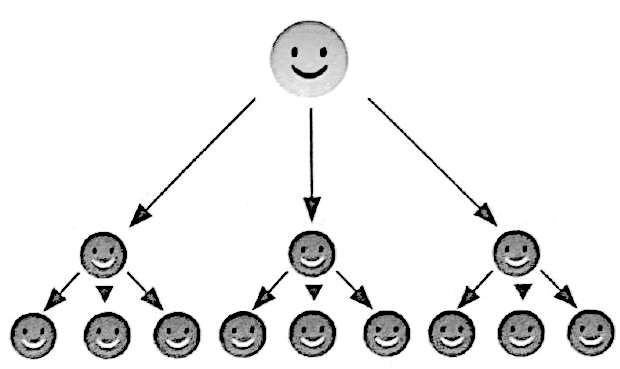
\includegraphics[width=0.3\textwidth]{assets/13-10.jpg}
                \end{center}
            \end{multicols}
            
            \item Sweetheart Sugar Factory produced $50,000$ tons of sugar this year (the first year). If the production increases by $10\%$ each year compared to the previous year, find the production for the 5th year and the total production for these 5 years.
            
            \item When Xiaohua was in high school, her mother gave her RM $200$ pocket money each month. Xiaohua's mother asked her to consider the following two plans:
            
            First plan: In each subsequent year, the monthly pocket money increases by RM $20$ compared to the previous year.

            Second plan: In each subsequent year, the monthly pocket money increases by $8.8\%$ compared to the previous year.
            \begin{enumerate}
                \item Under each plan, calculate the monthly pocket money Xiaohua receives when she is in the third year of high school. Which one is more?
                
                \item Under each plan, calculate the total pocket money Xiaohua receives during six years of secondary school. Which one is more?
            \end{enumerate}
            
            \item A ball falls vertically from a height of $2$ meters to the ground. After hitting the ground, it rebounds vertically, reaching $80\%$ of its original height, and then falls back down. This process repeats, with each subsequent rebound reaching $80\%$ of the previous height. How far does the ball travel in total?
        \end{enumerate}

        \section{Compound Interest and Annuities}

        Back in junior high, we learned about simple interest calculations, but in real life, interest is typically calculated using \text{compound interest}. Suppose you open a bank account and deposit RM $p$, then leave it without withdrawing. The bank's \text{annual interest rate} is $r\%$, compounded annually. After one year, you'll receive interest of RM $p \times \dfrac{r}{100}$. Adding this to the \text{principal} RM $p$, your total deposit (principal plus interest) becomes:
        $$
        \text{RM } p \times \left(1+\dfrac{r}{100}\right)
        $$

        \vspace{-1em}
        When settling interest after two years, it's calculated based on the deposit from one year earlier, i.e., RM $p \times \left(1+\dfrac{r}{100}\right)$ as the principal. Therefore, the deposit after two years becomes:
        $$
        \text{RM } p \times \left(1+\dfrac{r}{100}\right) \times \left(1+\dfrac{r}{100}\right)
        $$

        \vspace{-1em}
        Similarly, the deposit after three years becomes:
        $$
        \text{RM } p \times \left(1+\dfrac{r}{100}\right) \times \left(1+\dfrac{r}{100}\right) \times \left(1+\dfrac{r}{100}\right)
        $$

        \vspace{-1em}
        And so on. The deposit after $n$ years becomes:
        $$
        \text{RM } p \times \underbrace{\left(1+\dfrac{r}{100}\right) \times \left(1+\dfrac{r}{100}\right) \times \cdots \times \left(1+\dfrac{r}{100}\right)}_{n \text{ terms}} = \text{RM } p \times \left(1+\dfrac{r}{100}\right)^n
        $$

        \vspace{-1em}
        If $\text{RM } a_n$ is the deposit after $n$ years, then $\left\{a_n\right\}$ forms a geometric sequence with common ratio $\left(1+\dfrac{r}{100}\right)$.

        Suppose the total deposit is $A$, with an annual interest rate of $r\%$. Then, the total deposit $A=p\left(1+\dfrac{r}{100}\right)^n$ or $p(1+r\%)^n$, where $p$ is also known as the \text{present value}.

        For some deposits, interest is not calculated annually but rather semi-annually, quarterly, monthly, or daily, corresponding to 2, 4, 12, or 365 times per year respectively. If the principal is RM $p$, the annual interest rate is $r\%$, and the interest is compounded $m$ times per year, then each time it's calculated using an interest rate of $\dfrac{r}{m}\%$. In total, interest is compounded $nm$ times after $n$ years. Therefore, the \textbf{accumulated value} after $n$ years is:
        
        \begin{info}[Compound Interest Formula]
            $$
            \text{Accumulated value} = \text{RM }p\left(1+\dfrac{r}{\dfrac{100}{m}}\right)^{nm}
            $$
        \end{info}

        \begin{question}
            Xiao Hua deposited RM $50,000$ into the bank, with an annual interest rate of $4\%$, compounded annually. If he does not withdraw the principal or interest, find the accumulated value after 15 years.

            \sol{}

            \vspace{-1em}
            \noindent Given that $p = 50,000$, $r = 4$, $n = 15$,
            \vspace{-1em}
            \begin{flalign*}
                \text{Accumulated value} &= 50,000 \times \left(1+\dfrac{4}{100}\right)^{15} = \text{RM } 90,047.18 &
            \end{flalign*}
        \end{question}

        \begin{question}
            Given that the principal is RM $100,000$, with an annual interest rate of $5\%$, compounded semi-annually, calculate the interest after $5$ years.

            \sol{}
            \vspace{-1em}
            \begin{flalign*}
                5 \text { years of interest } & =\text { Accumulated value }- \text { Principal } \\
                & =100000 \times\left(1+\dfrac{2.5}{100}\right)^{10}-100000 \\
                & =128008.45-100000 \\
                & =\text { RM } 28,008.45 &
            \end{flalign*}
            \vspace{-3em}
        \end{question}

        \begin{question}
            Xiao Fang deposits RM $5,000$ every year. If the annual interest rate is $3.5\%$, compounded annually, calculate the total amount after $20$ years.

            \sol{}
            
            \vspace{-1em}
            \noindent The accumulated value after $20$ years
            \vspace{-1em}
            \begin{flalign*}
                & =5000\left(1+\dfrac{3.5}{100}\right)^{20}+5000\left(1+\dfrac{3.5}{100}\right)^{19}+5000\left(1+\dfrac{3.5}{100}\right)+\cdots+5000\left(1+\dfrac{3.5}{100}\right) &\\
                & =5000\left(1.035+1.035^2+1.035^3+\cdots+1.035^{20}\right) \\
                & =5000 \times \dfrac{1.035\left(1-1.035^{20}\right)}{1-1.035} \\
                & =\text { RM } 146,347.35
            \end{flalign*}
        \end{question}

        \vspace{-2em}
        \begin{question}
            Given that the principal is RM $100,000$, the annual interest rate is $5.5\%$, compounded annually. How many years will it take for the total amount to exceed RM $150,000$?

            \sol{}

            \vspace{-1em}
            \noindent Let the number of years required be $n$ for the total amount to exceed RM $150,000$.
            \begin{flalign*}
                    100000\left(1+\dfrac{5.5}{100}\right)^n & >150000 &\\
                    1.055^n & >1.5 \\
                    \lg (1.055)^n & >\lg 1.5 \\
                    n & >\dfrac{\lg 1.5}{\lg 1.055} \\
                    n & >7.573
            \end{flalign*}

            \vspace{-2em}
            \noindent $\therefore$ It will take at least $8$ years for the total amount to exceed RM $150,000$.
        \end{question}
        \vspace{-2em}
        \begin{question}
            Given an annual interest rate of $6\%$, compounded annually, with interest settled annually, and interest of RM $15,281.28$ after $3$ years, find the principal amount.
            
            \sol{}

            \vspace{-1em}
            \noindent Let the principal be $p$.
            \begin{flalign*}
                p\left(1+\dfrac{6}{100}\right)^{3}-p & =15281.28 \\
                1.191016 p-p & =15281.28 &\\
                p & =80000
            \end{flalign*}

            \vspace{-2em}
            \noindent $\therefore$ The principal amount is RM $80,000$.
        \end{question}

        \newpage
        \subsection*{Annuities and Present Value}
        An \text{annuity} refers to a series of equal payments made or received at regular intervals under a certain contract. Examples include various instalment payments, rent, insurance premiums, instalment loan repayments, etc. The present value of an annuity is the total present value of all payments after putting the annual interest rate and the number of periods into consideration.

        If the annual interest rate is $r\%$, and the annuity is RM $A$, with payments made annually, using the formula $A=p(1+r\%)^{n}$, we can determine that the present value at year $n$ is $A(1+r\%)^{-n}$, where $n$ represents the number of periods. Therefore, the present value of the payment in the first year is $\dfrac{A}{1+r\%}$, in the second year is $\dfrac{A}{(1+r\%)^{2}}$, and so on.

        The present value of an annuity paid for $n$ years starting from the current year is:
        \begin{flalign*}
            \text{Present value of annuity} &= \dfrac{A}{1+r\%} + \dfrac{A}{(1+r\%)^{2}} + \cdots + \dfrac{A}{(1+r\%)^{n}} \\
            & =A\left[\dfrac{1}{1+r \%}+\dfrac{1}{(1+r \%)^2}+\cdots+\dfrac{1}{(1+r \%)^n}\right] \\
            & =A\left[\dfrac{1}{1+r \%} \times \dfrac{1-\dfrac{1}{(1+r \%)^n}}{1-\dfrac{1}{1+r \%}}\right] \\
            & =\dfrac{A}{r \%}\left[1-\dfrac{1}{(1+r \%)^n}\right]
        \end{flalign*}
        
        An annuity is not limited to paying only once per year.

        \begin{info}[Additional Information:]
            
            \noindent As $n$ approaches infinity, in the case of \text{perpetuity}, where payments are made continuously without end, $\dfrac{1}{(1+r\%)^{n}}$ approaches $0$. Thus, the present value formula for perpetuity is $\dfrac{A}{r\%}$.
        \end{info}

        \begin{question}
            Given an annuity of RM $1,500$, an annual interest rate of $5\%$, payments made annually, and continuous payments for $20$ years, we want to find the present value.

            \sol{}

            \noindent Given that $n = 20$, $A = \text{RM } 1,500$, $r = 5$,
            \begin{flalign*}
                    \text { Present value } & =\dfrac{1500}{5 \%}\left(1-\dfrac{1}{(1+5 \%)^{20}}\right) &\\
                    & =\dfrac{1500}{0.05}(0.62311) \\
                    & =\text{RM } 18,693.32
            \end{flalign*}
        \end{question}

        \newpage
        \begin{question}
            Given an annuity of RM $2,000$, an annual interest rate of $6\%$, and payments made once per year, how many years are needed for the present value to exceed RM $20,000$?

            \sol{}

            \noindent Let the number of years required be $n$ for the present value to exceed RM $20,000$.
            \begin{flalign*}
                \dfrac{2000}{6 \%}\left[1-\dfrac{1}{(1+6 \%)^n}\right] & >20000 &\\
                \left(1-\dfrac{1}{1.06^n}\right) & >0.6 \\
                \dfrac{1}{1.06^n} & <0.4 \\
                1.06^n & >2.5 \\
                n \lg 1.06 & >\lg 2.5 \\
                n & >\dfrac{\lg 2.5}{\lg 1.06} \\
                n & >15.73
            \end{flalign*}
            $\therefore$ It will take at least $16$ years for the present value to exceed RM $20,000$.

        \end{question}

        \practice{13.4}
        \begin{enumerate}
            \item Xiaofang deposited RM $2,000$ in the bank at an annual interest rate of $4\%$, compounded annually. She withdrew all the savings after ten years. How much money can she withdraw?
            
            \item Xiaoyu deposited RM $1,000$ in the bank with an annual interest rate of $3.6\%$. Calculate Xiaoyu's total deposit after one year in the following scenarios:
            \begin{enumerate}
                \item Interest compounded annually;
                \item Interest compounded semi-annually;
                \item Interest compounded quarterly.
            \end{enumerate}
        \end{enumerate}

        \newpage
    \exercise{13.4}
    \begin{enumerate}
        \item Given a principal of $\mathrm{RM} 80,000$ and an annual interest rate of $5\%$, compounded annually, find the total amount of principal and interest after 10 years.

        \item Someone deposits a sum of money with a compound interest rate of $6\%$, compounded annually. After $3$ years, the interest earned is RM $955.08$. Find the amount of the deposit.
        
        \item Deposit RM $80,000$ into a financial company with an annual interest rate of $5.5\%$, compounded quarterly. Find the accumulated value after $5$ years.

        \item Prove that with a compound interest rate of $5\%$, compounded annually, the accumulated value will exceed twice the principal after $15$ years.

        \item Given a principal of RM $20,000$ and an annual interest rate of $6\%$, compounded annually, how many years are needed for the accumulated value to exceed RM $200,000$?

        \item Given a principal of RM $120,000$ and a compound interest rate of $4.5\%$ compounded annually, how many years are needed to earn RM $50,652.07$ in interest?

        \item Someone deposits RM $2,500$ annually. If the annual interest rate is $4\%$, compounded annually, find the total principal and interest after $15$ years.

        \item If the present value is RM $15,443.46$ and the annual interest rate is $5\%$, find the continuous annuity for $10$ years.

        \item Given an annuity of RM $5,000$, an annual interest rate of $5\%$, with annual payments for $25$ years, find the present value of the annuity and the present value of if it is a perpetuity.

        \item Given an annuity of RM $2,500$, an annual interest rate of $4.5\%$, with annual payments, how many years are needed for the present value to exceed RM $30,000$?
    \end{enumerate}

    \section{Special Summation of Series}

    Let's start by observing the formula for the sum of the first \( n \) natural numbers:
    \[
    1 + 2 + 3 + \cdots + n = \dfrac{n(n+1)}{2}
    \]

    \vspace{-2em}
    Now, let's examine the sum of squares of the first \( n \) natural numbers, denoted as \( \displaystyle\sum_{k=1}^{n} k^{2} = 1^{2} + 2^{2} + 3^{2} + \cdots + n^{2} \).

    First, we notice that:
    \[
    \begin{aligned}
    (n+1)^{3} &= n^{3} + 3n^{2} + 3n + 1 \\
    (n+1)^{3} - n^{3} &= 3n^{2} + 3n + 1
    \end{aligned}
    \]
    
    \vspace{-2em}
    \begin{center}
        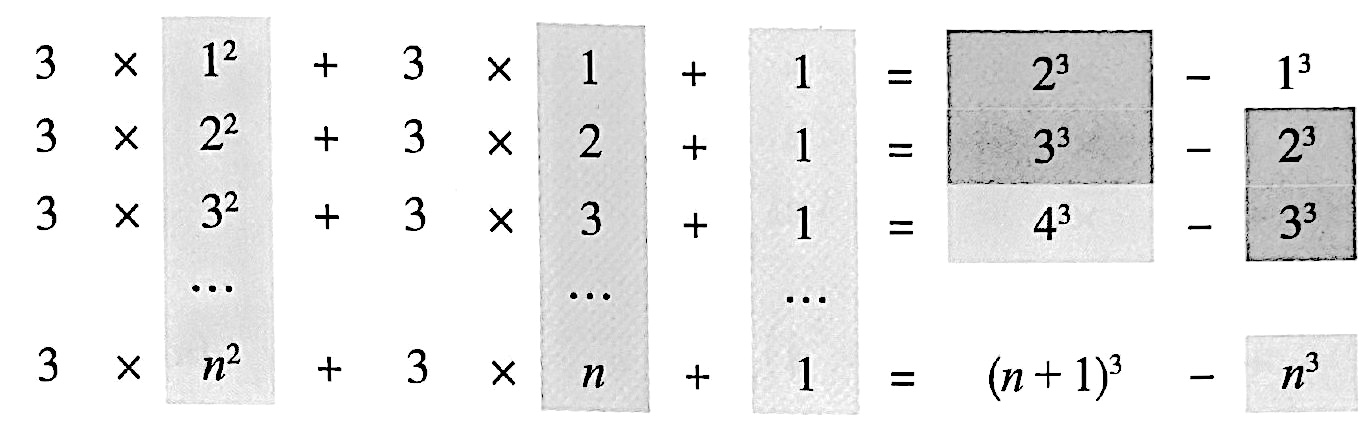
\includegraphics[width=0.7\textwidth]{assets/13-11.jpg}
    \end{center}
    \newpage
    Adding these $n$ equations together, we get:
    \begin{flalign*}
        3 \sum_{k=1}^{n} k^{2}+3 \sum_{k=1}^{n} k+\sum_{k=1}^{n} 1 & =(n+1)^{3}-1 \\
        3 \sum_{k=1}^{n} k^{2}+3 \times \dfrac{n(n+1)}{2}+n & =n^{3}+3 n^{2}+3 n \\
        3 \sum_{k=1}^{n} k^{2} & =n^{3}+3 n^{2}+2 n-\dfrac{3 n(n+1)}{2} \\
        & =n(n+1)(n+2)-\dfrac{3 n(n+1)}{2} \\
        & =\dfrac{n(n+1)(2 n+4-3)}{2} \\
        \therefore \sum_{k=1}^{n} k^{2} & =\dfrac{n(n+1)(2 n+1)}{6}
            \end{flalign*}
            \begin{info}[Sum of the First \( n \) Squares]
                \[
                \sum_{k=1}^{n} k^{2} = \dfrac{n(n+1)(2n+1)}{6}
                \]
            \end{info}

            Next, let's inspect $ \displaystyle\sum_{k=1}^{n} k^{3} = 1^{3} + 2^{3} + 3^{3} + \cdots + n^{3} $. From
            \begin{align*}
                (n+1)^{4} & =n^{4}+4 n^{3}+6 n^{2}+4 n+1 &&&&&&&&&&&& \\
                (n+1)^{4}-n^{4} & =4 n^{3}+6 n^{2}+4 n+1
            \end{align*}

            \vspace{-2em}
            \begin{center}
                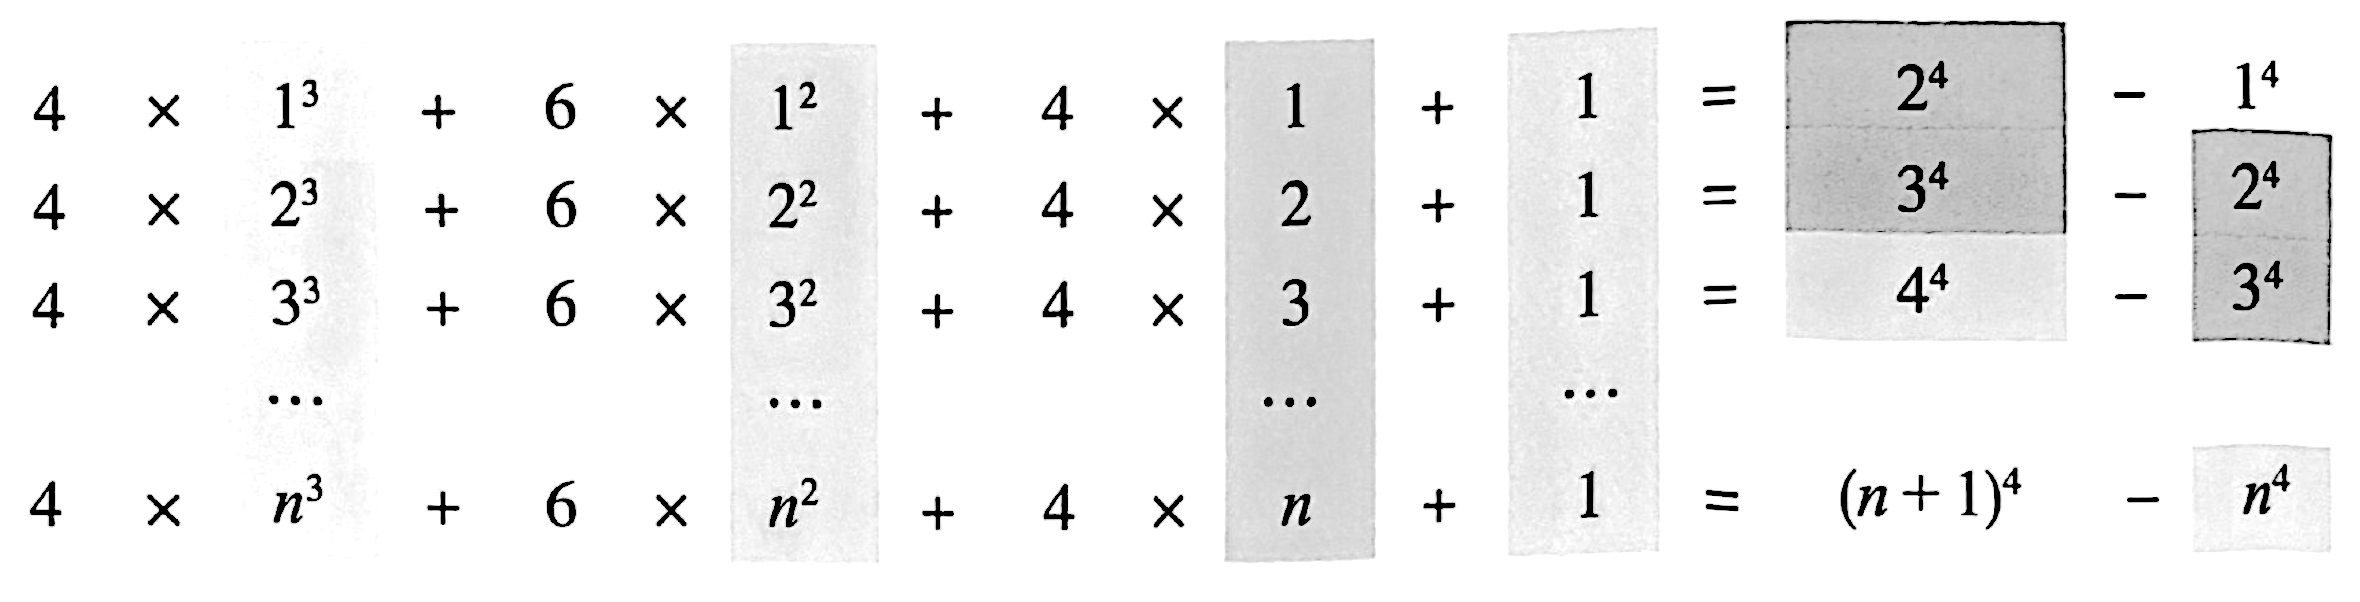
\includegraphics[width=0.7\textwidth]{assets/13-12.png}
            \end{center}
            \vspace{-1em}
            Adding these $n$ equations together, we get:
            \begin{flalign*}
            4 \sum_{k=1}^{n} k^{3}+6 \sum_{k=1}^{n} k^{2}+4 \sum_{k=1}^{n} k+\sum_{k=1}^{n} 1&=(n+1)^{4}-1 \\
            4 \sum_{k=1}^{n} k^{3}+6 \times \dfrac{n(n+1)(2 n+1)}{6}+4 \times \dfrac{n(n+1)}{2}+n&=n^{4}+4 n^{3}+6 n^{2}+4 n 
            \end{flalign*}
            \vspace{-2em}
            \begin{flalign*}
            4 \sum_{k=1}^{n} k^{3}&=n^{4}+4 n^{3}+6 n^{2}+4 n-\left(2 n^{3}+3 n^{2}+n\right)-\left(2 n^{2}+2 n\right)-n \\
            & =n^{4}+2 n^{3}+n^{2} \\
            & =n^{2}(n+1)^{2} \\
            \therefore \sum_{k=1}^{n} k^{3}&=\dfrac{n^{2}(n+1)^{2}}{4} \\
            & =\left[\dfrac{n(n+1)}{2}\right]^{2}
            \end{flalign*}

            \begin{info}[Sum of the First \( n \) Cubes]
                \[
                \sum_{k=1}^{n} k^{3} = \left[\dfrac{n(n+1)}{2}\right]^{2}
                \]
            \end{info}

            \begin{question}
                Find $1 \times 2+2 \times 3+3 \times 4+\cdots+n(n+1)$.

                \sol{}
                \begin{flalign*}
                    1 \times 2+2 \times 3+3 \times 4+\cdots+n(n+1) & =\sum_{k=1}^n k(k+1) &\\
                    & =\sum_{k=1}^n\left(k^2+k\right) \\
                    & =\sum_{k=1}^n k^2+\sum_{k=1}^n k \\
                    & =\dfrac{n(n+1)(2 n+1)}{6}+\dfrac{n(n+1)}{2} \\
                    & =\dfrac{n(n+1)(2 n+1+3)}{6} \\
                    & =\dfrac{n(n+1)(n+2)}{3}
                \end{flalign*}
            \end{question}

            \begin{question}
                Find the sum of the first $n$ terms of the series $1^{3}+3^{3}+5^{3}+\cdots$.

                \sol{}

                \noindent The $n$th term of the series $1^{3}+3^{3}+5^{3}+\cdots$ is given by \(a_{n}=(2 n-1)^{3}\).

                \noindent\textbf{Approach 1:}
                \begin{flalign*}
                    & 1^{3}+3^{3}+5^{3}+\cdots+(2 n-1)^{3} &\\
                    & =\sum_{k=1}^{n}(2 k-1)^{3} \\
                    & =\sum_{k=1}^{n}\left(8 k^{3}-12 k^{2}+6 k-1\right) \\
                    & =8 \sum_{k=1}^{n} k^{3}-12 \sum_{k=1}^{n} k^{2}+6 \sum_{k=1}^{n} k-\sum_{k=1}^{n} 1 \\
                    & =8 \times \dfrac{n^{2}(n+1)^{2}}{4}-12 \times \dfrac{n(n+1)(2 n+1)}{6}+6 \times \dfrac{n(n+1)}{2}-n \\
                    & =n\left(2 n^{3}+4 n^{2}+2 n-4 n^{2}-6 n-2+3 n+3-1\right) \\
                    & =n\left(2 n^{3}-n\right) \\
                    & =n^{2}\left(2 n^{2}-1\right)
                \end{flalign*}
            \end{question}

            \newpage
            \setcounter{Question}{38}
            \begin{question}
                \textbf{Approach 2:}
                \begin{flalign*}
                    2^{3}+4^{3}+6^{3}+\cdots+(2 n)^{3}&=2^{3}\left(1^{3}+2^{3}+3^{3}+\cdots+n^{3}\right) &\\
                    & =8 \times \dfrac{n^{2}(n+1)^{2}}{4} \\
                    & =2 n^{2}(n+1)^{2} 
                \end{flalign*}
                \vspace{-3.5em}
                \begin{flalign*}
                    & 1^{3}+3^{3}+5^{3}+\cdots+(2 n-1)^{3} &\\
                    & =\left[1^{3}+2^{3}+3^{3}+4^{3}+\cdots+(2 n-1)^{3}+(2 n)^{3}\right]-\left[2^{3}+4^{3}+\cdots+(2 n)^{3}\right] \\
                    & =\dfrac{(2 n)^{2}(2 n+1)^{2}}{4}-2 n^{2}(n+1)^{2} \\
                    & =n^{2}\left(4 n^{2}+4 n+1-2 n^{2}-4 n-2\right) \\
                    & =n^{2}\left(2 n^{2}-1\right)
                \end{flalign*}
            \end{question}

            \begin{question}
                Given that $\dfrac{1}{n(n+1)}=\dfrac{1}{n}-\dfrac{1}{n+1}$. Find $\displaystyle\sum_{k=1}^{n} \dfrac{1}{k(k+1)}$.
                \begin{flalign*}
                    \sum_{k=1}^n \dfrac{1}{k(k+1)}&=\dfrac{1}{1 \times 2}+\dfrac{1}{2 \times 3}+\dfrac{1}{3 \times 4}+\cdots+\dfrac{1}{n(n+1)} &\\
                    & =\left(1-\dfrac{1}{2}\right)+\left(\dfrac{1}{2}-\dfrac{1}{3}\right)+\left(\dfrac{1}{3}-\dfrac{1}{4}\right)+\cdots+\left(\dfrac{1}{n-1}-\dfrac{1}{n}\right)+\left(\dfrac{1}{n}-\dfrac{1}{n+1}\right) \\
                    & =1-\dfrac{1}{n+1} \\
                    & =\dfrac{n}{n+1}
                \end{flalign*}
            \end{question}

        \begin{question}
            Find sum of the series $\dfrac{1}{2}+\dfrac{3}{4}+\dfrac{5}{8}+\dfrac{7}{16}+\cdots+\dfrac{2 n-1}{2^{n}}$.

            \sol{}

            \noindent This series is formed by the product of corresponding terms of an arithmetic sequence $1, 3, 5, 7, \cdots$ and a geometric sequence $\dfrac{1}{2}, \dfrac{1}{4}, \dfrac{1}{8}, \dfrac{1}{16}, \cdots$. Series like this are usually summed using the following method.

            \noindent Let$\begin{aligned}[t] S_n & =\dfrac{1}{2}+\dfrac{3}{2^2}+\dfrac{5}{2^3}+\dfrac{7}{2^4}+\cdots+\dfrac{2 n-1}{2^n}\ \cdots\ (1) \\ \dfrac{1}{2} S_n & =\dfrac{1}{2^2}+\dfrac{3}{2^3}+\dfrac{5}{2^4}+\dfrac{7}{2^5}+\cdots+\dfrac{2 n-1}{2^{n+1}}\ \cdots\ (2)\end{aligned}$
        \end{question}

        \setcounter{Question}{40}
        \begin{question}
            $(1) - (2)$ gives $\begin{aligned}[t] \dfrac{1}{2} S_n & =\dfrac{1}{2}+\left(\dfrac{2}{2^2}+\dfrac{2}{2^3}+\dfrac{2}{2^4}+\cdots+\dfrac{2}{2^n}\right)-\dfrac{2 n-1}{2^{n+1}} \\ & =\dfrac{1}{2}+\left(\dfrac{1}{2}+\dfrac{1}{2^2}+\dfrac{1}{2^3}+\cdots+\dfrac{1}{2^{n-1}}\right)-\dfrac{2 n-1}{2^{n+1}} \\ & =\dfrac{1}{2}+1-\dfrac{1}{2^{n-1}}-\dfrac{2 n-1}{2^{n+1}} \\ S_n & =3-\dfrac{2 n+3}{2^n}\end{aligned}$
        \end{question}

        \practice{13.5}
        \begin{enumerate}
            \item Find the sum of $10^{2}+11^{2}+12^{2}+\cdots+50^{2}$.

            \item Find the sum of $1 \times 2 \times 3+2 \times 3 \times 4+3 \times 4 \times 5+\cdots+n(n+1)(n+2)$.
            \item Find the sum of the first $n$ terms of the series $1+3+5+7+\cdots$.
            \item Find the sum of the first $n$ terms of the series $1^{2}+3^{2}+5^{2}+7^{2}+\cdots$.
        \end{enumerate}

        \exercise{13.5}
        \begin{enumerate}
            \item Find the sum of the first $20$ terms of the series $2 \dfrac{1}{2}+4 \dfrac{1}{4}+8 \dfrac{1}{8}+\cdots$.

            \item Given the sequence $\left\{a_{n}\right\}$ where the $n$th term is $a_{n}=2 n-1+\left(\dfrac{2}{3}\right)^{n}$, find the sum of the first $n$ terms of this sequence.
            
            \item Find the sum of the first $n$ terms of the series $1 \dfrac{1}{3}+4 \dfrac{1}{9}+7 \dfrac{1}{27}+\cdots$.
            
            \item Find the sum of the infinite series $\dfrac{1}{3}+\dfrac{4}{9}+\dfrac{7}{27}+\dfrac{10}{81}+\cdots$.
            
            \item Find the sum of the first $n$ terms of the series $x+5 x^{2}+9 x^{3}+13 x^{4}+\cdots$. 
            
            Hence, if $|x|<1$, find the sum of this series to infinity.

            \item Find the sum of the first $n$ terms of the series $\dfrac{1}{1 \times 4}+\dfrac{1}{4 \times 7}+\dfrac{1}{7 \times 10}+\cdots$.
            
            \item Given $\dfrac{1}{(3 n-2)(3 n+1)(3 n+4)}=\dfrac{1}{18(3 n-2)}-\dfrac{1}{9(3 n+1)}+\dfrac{1}{18(3 n+4)}$, find the sum of the first $n$ terms of the series $\dfrac{1}{1 \times 4 \times 7}+\dfrac{1}{4 \times 7 \times 10}+\dfrac{1}{7 \times 10 \times 13}+\cdots$, and find the sum of this series to infinity.
            
            \item Without using a calculator, find the value of $1-2 \times 3+3 \times 3^{2}-4 \times 3^{3}+5 \times 3^{4}-\cdots+11 \times 3^{10}$.
            
            \item Find the sum of the series $\dfrac{1}{\sqrt{1}+\sqrt{3}}+\dfrac{1}{\sqrt{3}+\sqrt{5}}+\dfrac{1}{\sqrt{5}+\sqrt{7}}+\cdots+\dfrac{1}{\sqrt{119}+\sqrt{121}}$.
            
            \newpage
            \item Find the value of the following expressions:
            \begin{tasks}[label=(\alph*)](2)
                \task $\displaystyle\sum_{k=1}^{8}(2 k-1)^{2}$
                \task $\displaystyle\sum_{k=6}^{12} k(k+2)$
                \task $\displaystyle\sum_{k=1}^{10}(2 k-1)^{3}$
                \task $\displaystyle\sum_{k=3}^{10} k\left(k^{2}-k+1\right)$
            \end{tasks}

            \item Given that the $n$th term of a sequence is $a_{n}=3 n^{2}+n$, find the sum of the first $n$ terms of this sequence.
            
            \item Find the sum of the first $n$ terms of the series $1 \times 3+2 \times 7+3 \times 11+4 \times 15+\cdots$.
            
            \item Find the sum of the first $n$ terms of the series $1 \times 4 \times 7+2 \times 5 \times 8+3 \times 6 \times 9+\cdots$.
            
            \item Given a sequence $\left\{a_{n}\right\}$ defined by $a_{1}=3$ and for $n \geq 2, a_{n}=a_{n-1}+2 n$,
            \begin{enumerate}
                \item Find the general formula for this sequence.
                \item Find the sum of the first $n$ terms of this sequence.
            \end{enumerate}
        \end{enumerate}

        \vspace{-2em}
        \revision{13}

        \vspace{-1em}
        \begin{enumerate}
            \item Given that the sum of the first $4$ terms of an arithmetic series is $28$, and the sum of the first $8$ terms is $48$, find the sum of the first $12$ terms.
            
            \item Find the sum of all integers from $1$ to $1000$ that are not divisible by $7$.
            
            \item Find the sum of all integers from $150$ to $300$ that are divisible by both $3$ and $5$.
            
            \item Find the sum of all natural numbers less than 300 that are divisible by $6$ but not by $8$.
            
            \item \parbox[t]{\textwidth}{
                \begin{center}
                    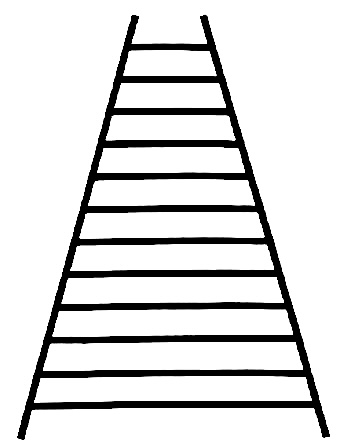
\includegraphics[width=0.15\textwidth]{assets/13-13.jpg}
                \end{center}
            }
            A ladder has a total of $12$ steps, with the top step being $33$ cm wide and the bottom step being $110$ cm wide. The widths of the steps form an arithmetic sequence.
            
            \begin{enumerate}
                \item Find the width of the $8^{th}$ step counting from the bottom.
            
                \item If the material for the horizontal beams of these ladders costs RM $2$ per meter, how much money is needed to manufacture all $12$ steps of the ladder?
            \end{enumerate}
            
            \item In the arithmetic series \(10+9\frac{1}{5}+8\frac{2}{5}+\cdots\), what is the position of the first negative term? Summing the terms from the first term up to which term will start to result in a negative sum?
            
            \item It is known that the $10^{th}$ term of an arithmetic series is $-23$, and the $25^{th}$ term is $22$.
            
            \begin{enumerate}
                \item From which term onwards are the terms positive?
            
                \item Up to which term, starting from the first term, is the sum positive?
            \end{enumerate}
            
            \item In a certain place, the rice yield was $100,000$ kilograms in $2015$, and it increased by $10\%$ every year thereafter. In which year will the cumulative yield reach $771,561$ kilograms?
            
            \item It is known that the interior angles of a convex polygon form an arithmetic sequence with a common difference of $5$, and the smallest angle is $120^{\circ}$. Find the number of sides of this polygon.
            
            \item \parbox[t]{\textwidth}{
                \begin{center}
                    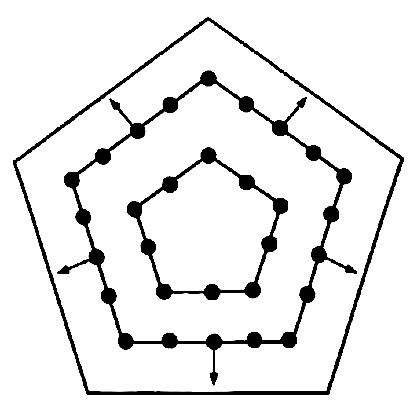
\includegraphics[width=0.2\textwidth]{assets/13-14.jpg}
                \end{center}
            }
            As shown in the diagram, there are several students forming a cheerleading formation in the shape of a regular pentagon, with the number of students per side increasing as you move outward from the center. It is known that there are $3$ students per side in the innermost circle, and the number of students per side increases by $2$ for each successive circle (i.e. the second circle has $5$ students per side, the third circle has $7$ students per side, and so on). How many students are there in the outermost circle (the $10^{th}$ circle)? How many students are there in total participating in the cheerleading performance?

            \item Given that the second term of an arithmetic sequence is $10$, and the sum of the first $3$ terms equals the sum of the first $10$ terms, determine from which term onwards the sequence becomes negative.
            
            \item Given that \(w, x, y, z\) form a geometric sequence and \(w+z=9, x+y=6\), find the common ratio of this sequence.
            
            \item Given that \(a, b, c\) are all positive numbers, in the sequence \(4, a, b, c, 64\), \(4, a, b\) form a geometric sequence, \(b, c, 64\) form a geometric sequence, but \(a, b, c\) form an arithmetic sequence. Find the values of \(a, b, c\).
            
            \item \parbox[t]{\textwidth}{
                \begin{center}
                    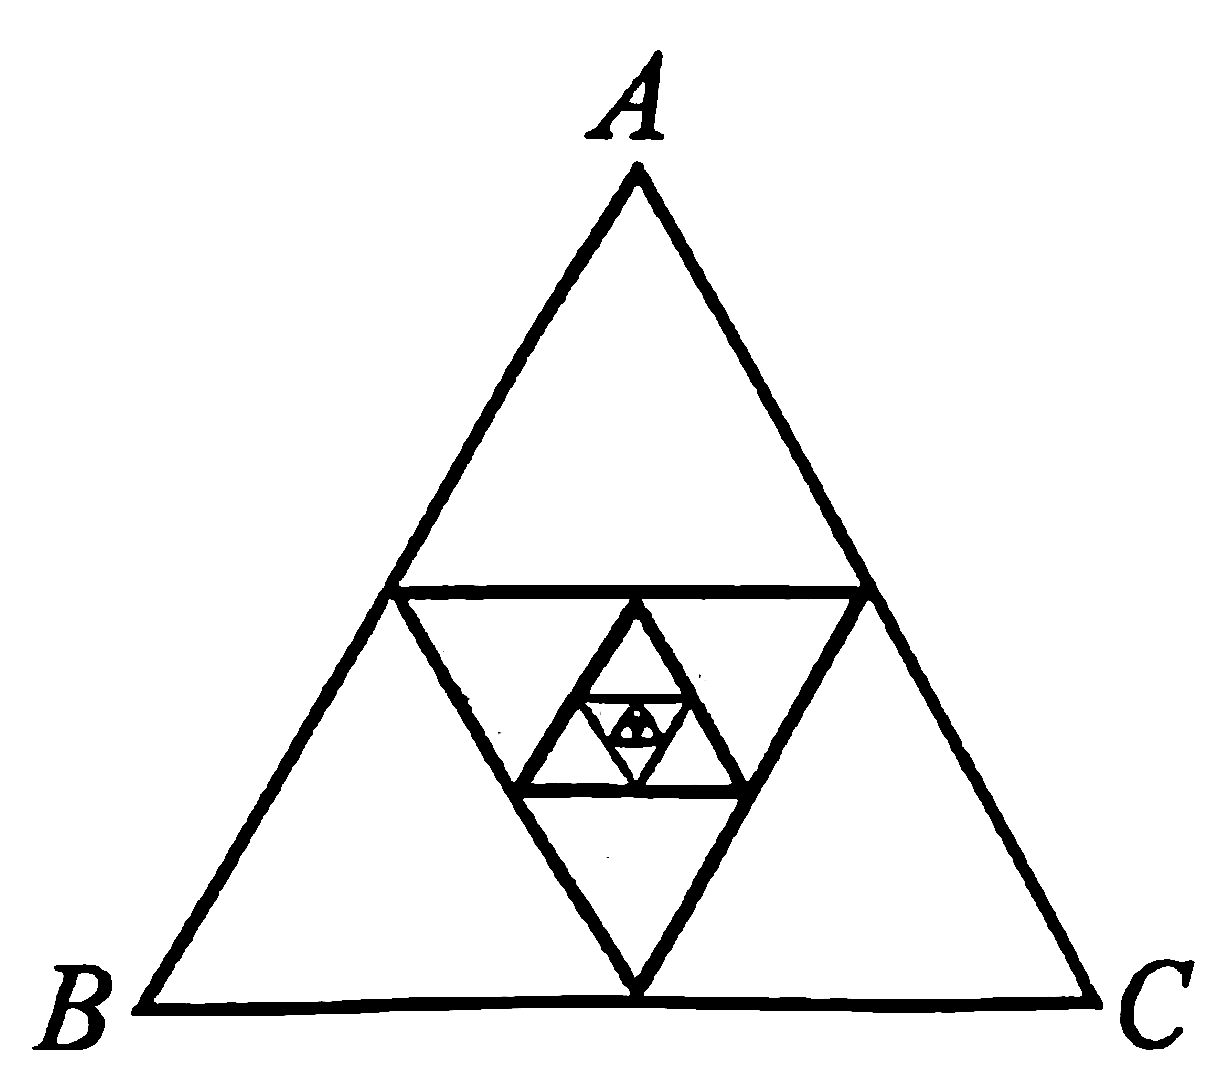
\includegraphics[width=0.2\textwidth]{assets/13-15.png}
                \end{center}
            }
            In the diagram, \(\triangle ABC\) is an equilateral triangle with area \(S\). Connecting the midpoints of its sides forms another triangle. Continuing this process infinitely, find the sum of the areas of all the triangles.
            
            \item If \(a, b, c\) are positive numbers and \(\log a, \log b, \log c\) form an arithmetic sequence, prove that \(a, b, c\) form a geometric sequence.
            
            \item Given that \(x, y, z\) form an arithmetic sequence, \(x, y, z+8\) form a geometric sequence, and \(x+y+z=18\), find the values of \(x, y, z\).
            
            \item Given that \(a, b, c\) form a geometric sequence and \(a+1, b+5, c+25\) also form a geometric sequence, find the ratio of \(a: b: c\).
            
            \item Given that \(x-3, x+1, 4x-2\) form a geometric sequence with a common ratio of \(r\), and the sum of these three numbers is \(S\), find \(r+S\).
            
            \item Given that the sum of the first \(n\) terms of a geometric series is $5$, and the sum of the first \(2n\) terms is $650$, find the sum of the first \(3n\) terms.
            
            \item Starting from $2005$, Xiaotian deposits RM $6,000$ into a bank at the beginning of each year with an annual interest rate of $3\%$, compounded semi-annually. If Xiaotian does not withdraw any principal or interest, what is the total amount of his deposit in the bank after depositing money at the beginning of $2020$?
            
            \item Given a principal of RM 75,000 with an annual interest rate of $4.5\%$, compounded quarterly, find the accumulated value after $10$ years.
            
            \item Xiaoxiang deposited a sum of money with an annual interest rate of $5.5\%$, compounded annually. After 5 years, the deposit increased by RM $2455.68$. Find the amount of the deposit.
            
            \item Given a principal of RM $120,000$ with an annual interest rate of $5\%$, compounded annually, how many years will it take for the accumulated value to exceed RM 250,000?
            
            \item If the present value is RM $22,939.84$ and the annual interest rate is $6\%$, find the annuity payable continuously for $20$ years.
            
            \item Given an annuity of RM 8,000 with an annual interest rate of $4.5\%$, paid annually for $15$ years, find the present value and the present value of perpetuity.
            
            \item Given an annuity of RM $4,500$ with an annual interest rate of $4\%$, paid annually, how many years will it take for the present value to exceed RM $50,000$?
            
            \item Xiao Ming, who has just entered university, plans to buy a computer worth RM $3,000$ using a loan and then repay it in instalments by working part-time. If Xiao Ming repays the loan once a month, clearing all the debt in $12$ instalments, and the monthly interest rate of the loan is $0.5\%$ compounded monthly, find the monthly instalment amount (rounded to the nearest integer).
            
            \item A brand laptop worth RM $2,500$ can be purchased in two instalment payment options:
            
            Option 1: Payment in $3$ installments, with one payment every $4$ months.
            
            Option 2: Payment in $6$ installments, with one payment every $2$ months.
            
            If the monthly interest rate is $0.6\%$, calculated on a compound interest basis, and the payment amount is the same each time, determine which payment option is more cost-effective.
            
            \item Find the sum of the first \(n\) terms of the series \(2\frac{1}{2}+5\frac{1}{4}+8\frac{1}{8}+11\frac{1}{16}+\cdots\).
            
            \item Given that \(S_{n}=[n(n+1)]^{2}\) is the sum of the first \(n\) terms of the sequence \(\{a_{n}\}\), find:
            \begin{enumerate}
                \item \(a_{n}\)
                \item \(\displaystyle\sum_{n=5}^{10} a_{n}\)
            \end{enumerate}
            
            \item Given that the sequence \(\{a_{n}\}\) satisfies \(a_{1}+2a_{2}+3a_{3}+\cdots+na_{n}=n^{2}(n+1)\), find \(a_{n}\) and \(a_{200}\).
            
            \item Given that the \(n\)th term of a sequence is \(a_{n}=n(n+1)(n+3)\), find the sum of the first \(n\) terms of this sequence.
            
            \item Find the sum of the first \(n\) terms of the series \(2 \times 5+5 \times 8+8 \times 11+11 \times 17+\cdots\).
        \end{enumerate}

\end{document}